\documentclass[12pt,a4paper]{report}
\usepackage[T1]{fontenc}
\usepackage{graphicx}
\usepackage{tikz}
\usetikzlibrary{positioning,shapes.geometric}
\usepackage{geometry}
\usepackage{hyperref}
\usepackage{enumitem}
\usepackage{booktabs}

\geometry{margin=1in}

\title{\textbf{Section X: Cybersecurity \& Cyber-Resilience Strategy for Sovereign Cloud/Edge Computing}}
\author{}
\date{}

\begin{document}

\hypersetup{pageanchor=false}
\maketitle
\hypersetup{pageanchor=true}

\tableofcontents
\newpage

\begin{figure}[!ht]
		\centering
		\resizebox{\textwidth}{!}{%
		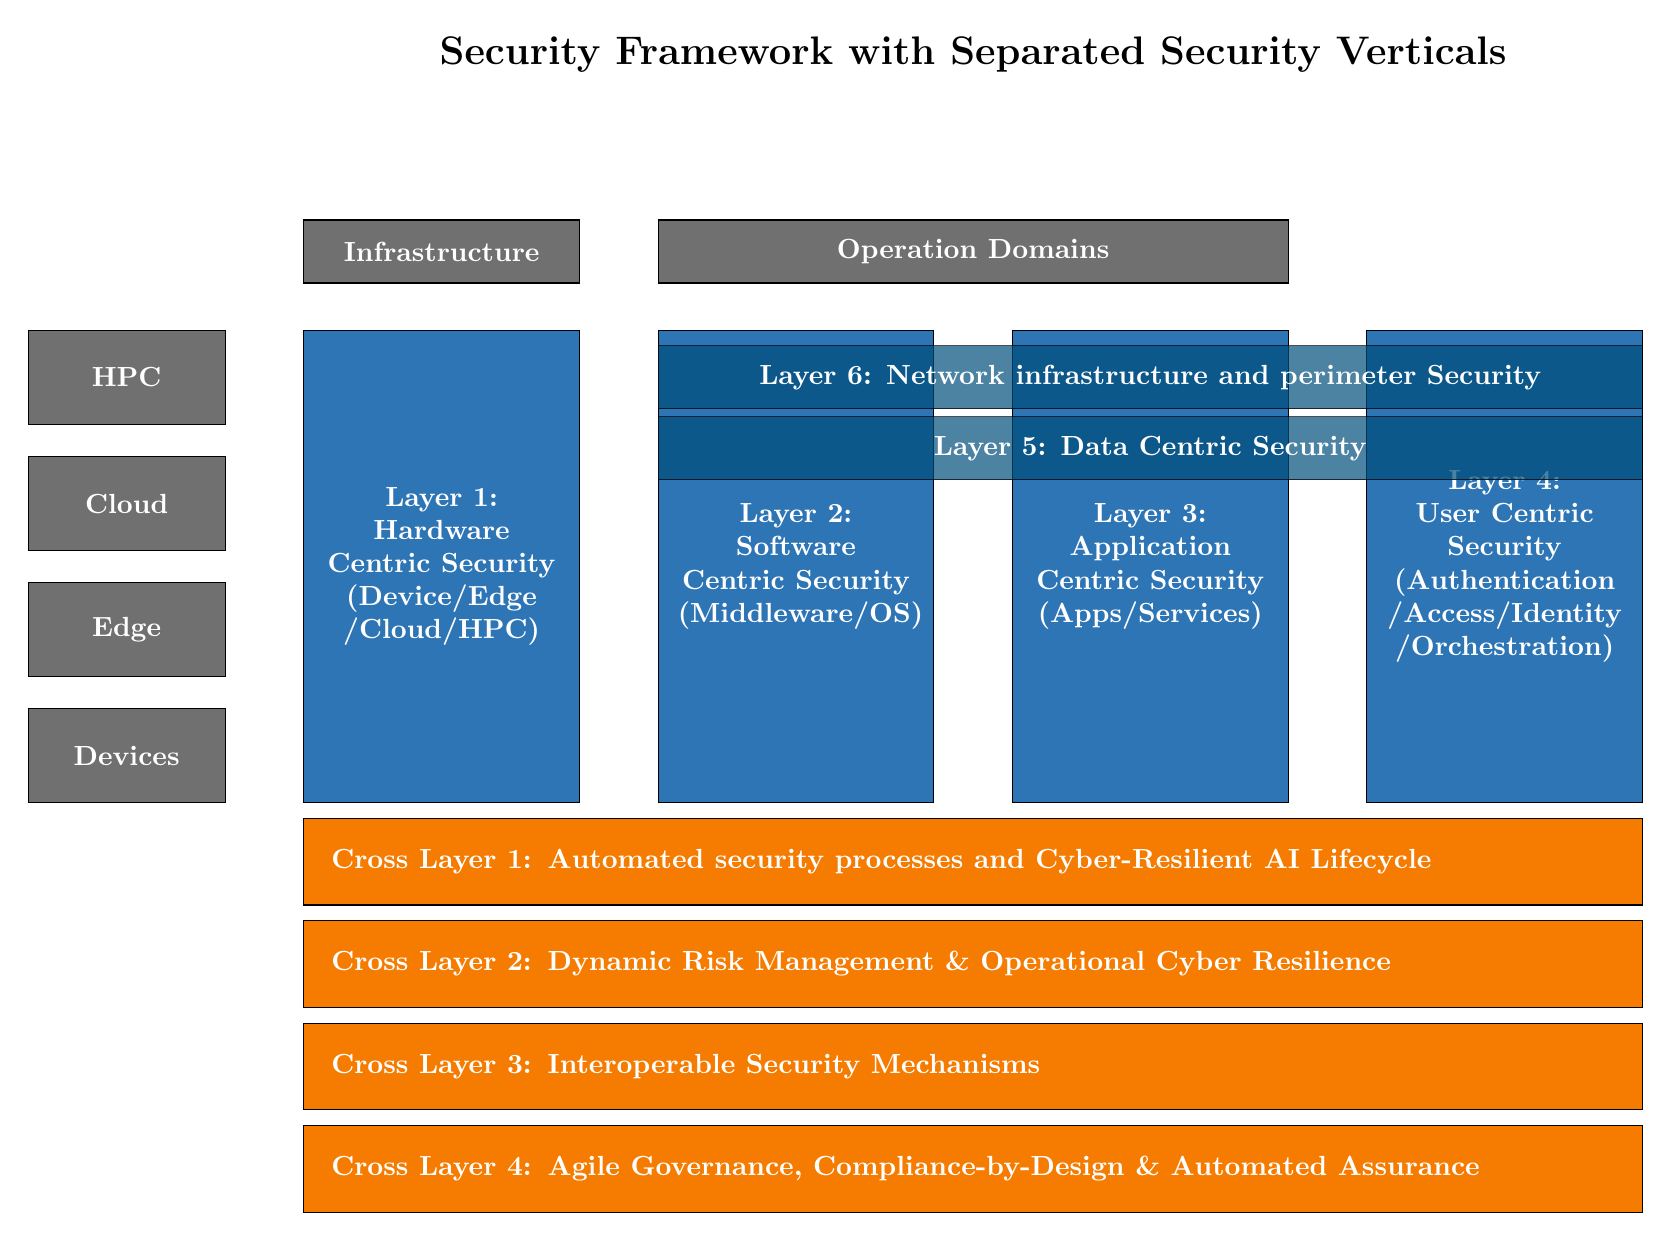
\begin{tikzpicture}[every node/.style={font=\small}]
			% Define colors
			\definecolor{archblue}{RGB}{46, 117, 182}
			\definecolor{sec_verticals_bg}{RGB}{245, 124, 0}
			\definecolor{env_bg}{RGB}{112, 112, 112}
			\definecolor{overlay}{RGB}{0, 77, 122}

			% Styles
			\tikzstyle{arch_col} = [fill=archblue, draw=black, text=white, font=\bfseries, minimum width=3.5cm, minimum height=6cm, align=center, text width=3cm]
			\tikzstyle{env_box} = [fill=env_bg, draw=black, text=white, font=\bfseries, minimum width=2.5cm, minimum height=1.2cm, align=center]
			\tikzstyle{top_tool} = [draw=black, fill=env_bg, text=white, minimum height=0.8cm, align=center, font=\bfseries]
			\tikzstyle{overlay_box} = [fill=overlay, draw=black, text=white, font=\bfseries, minimum height=0.8cm, align=center, opacity=0.7, text opacity=1]
			\tikzstyle{vertical_box} = [fill=sec_verticals_bg, draw=black, text=white, font=\bfseries, minimum width=17.0cm, minimum height=1.1cm, align=left, text width=16.3cm]

			% Column X positions
			\def\colone{-4.5}
			\def\coltwo{0}
			\def\colthree{4.5}
			\def\colfour{9}
            \pgfmathsetmacro{\layerSpanLeft}{\coltwo-1.75}
            \pgfmathsetmacro{\layerSpanRight}{\colfour+1.75}
            \pgfmathsetmacro{\layerSpanCenter}{(\layerSpanLeft+\layerSpanRight)/2}
            \pgfmathsetmacro{\layerSpanWidth}{\layerSpanRight-\layerSpanLeft}

			% Environment boxes (left)
			\node[env_box] at (-8.5, 2.4) {HPC};
			\node[env_box] at (-8.5, 0.8) {Cloud};
			\node[env_box] at (-8.5, -0.8) {Edge};
			\node[env_box] at (-8.5, -2.4) {Devices};

			% Main architecture columns representing layers
			\node[arch_col] (hw) at (\colone, 0) {Layer 1: \\ Hardware Centric Security \\ (Device/Edge\\ /Cloud/HPC)};
			\node[arch_col] (mw) at (\coltwo, 0) {Layer 2: \\ Software Centric Security \\ (Middleware/OS)};
			\node[arch_col] (app) at (\colthree, 0) {Layer 3: \\ Application Centric Security \\ (Apps/Services)};
			\node[arch_col] (user) at (\colfour, 0) {Layer 4: \\ User Centric Security \\ (Authentication\\ /Access/Identity\\ /Orchestration)};

			% Top tooling boxes
			\node[top_tool, minimum width=3.5cm] at (\colone, 4) {Infrastructure};
			\node[top_tool, minimum width=8cm] at (2.25, 4) {Operation Domains};

			% Arrows from tooling
			\draw[->, line width=2pt, white] (\colone, 3.5) -- (\colone, 3.1);
			\draw[->, line width=2pt, white] (2.25, 3.5) -- (2.25, 3.1);

			% Other layers as overlays/headers
			\node[overlay_box, minimum width=12.5cm] at (4.5, 1.5) {Layer 5: Data Centric Security};
            \node[overlay_box, minimum width=\layerSpanWidth cm] at (\layerSpanCenter, 2.4) {Layer 6: Network infrastructure and perimeter Security};

			% Separated vertical boxes
			\node[vertical_box] at (2.25, -3.75) {\textbf{Cross Layer 1: Automated security processes and Cyber-Resilient AI Lifecycle}};
			\node[vertical_box] at (2.25, -5.05) {\textbf{Cross Layer 2: Dynamic Risk Management \& Operational Cyber Resilience}};
			\node[vertical_box] at (2.25, -6.35) {\textbf{Cross Layer 3: Interoperable Security Mechanisms}};
			\node[vertical_box] at (2.25, -7.65) {\textbf{Cross Layer 4: Agile Governance, Compliance-by-Design \& Automated Assurance}};

			% Title
			\node[font=\Large\bfseries, anchor=center] at (2.25, 6.5) {Security Framework with Separated Security Verticals};

		\end{tikzpicture}%
		}
		\caption{Security Framework with separated security verticals in dedicated boxes.}
		\label{fig:security_framework_verticals_boxes}
	\end{figure}

    \begin{figure}[!ht]
    \centering
    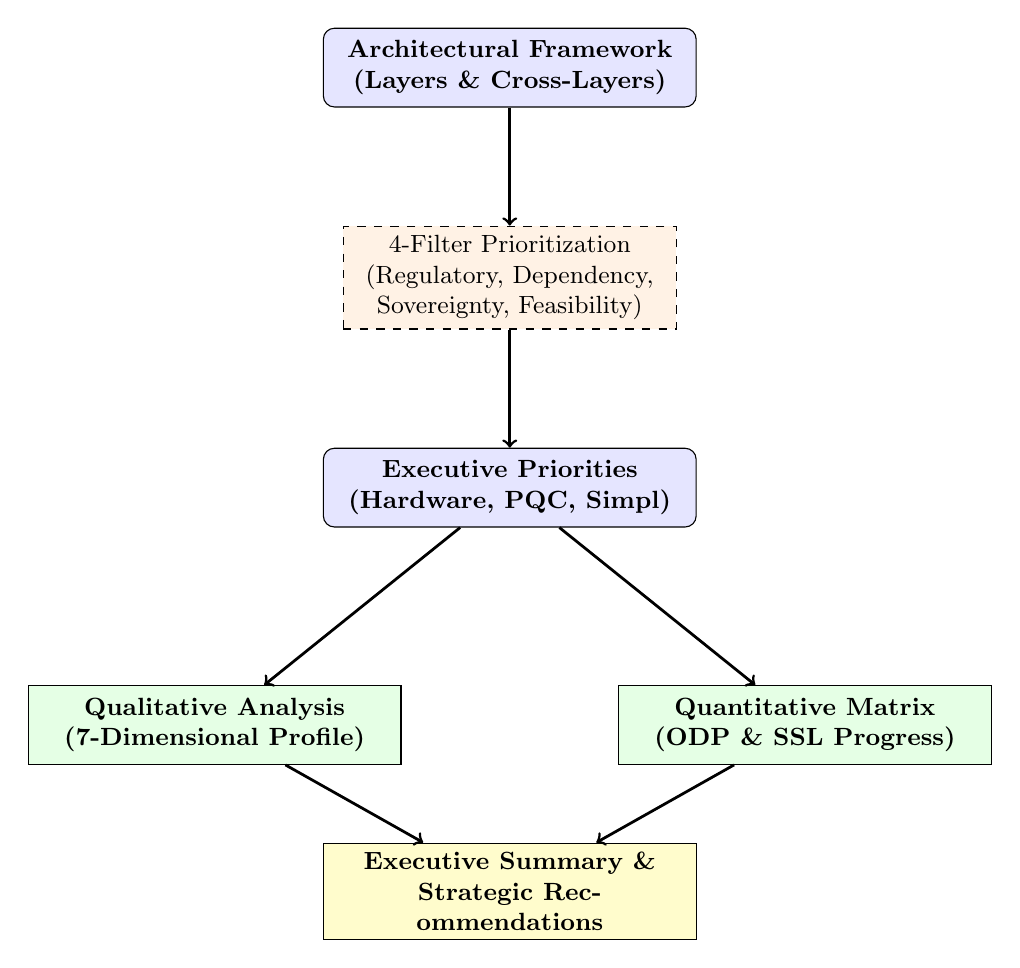
\begin{tikzpicture}[
        node distance=1.5cm,
        box/.style={draw, fill=blue!10, text width=4.5cm, align=center, minimum height=1cm, font=\small\bfseries, rounded corners},
        logic/.style={draw, fill=orange!10, text width=4cm, align=center, minimum height=1cm, font=\small, dashed},
        outcome/.style={draw, fill=green!10, text width=4.5cm, align=center, minimum height=1cm, font=\small\bfseries}
    ]

    % Nodes - Layer 1: Structure
    \node[box] (struct) {Architectural Framework \\ (Layers \& Cross-Layers)};
    
    % Nodes - Layer 2: Prompt/Methodology
    \node[logic, below=of struct] (filters) {4-Filter Prioritization \\ (Regulatory, Dependency, \\ Sovereignty, Feasibility)};
    
    % Nodes - Layer 3: Priorities
    \node[box, below=of filters] (priorities) {Executive Priorities \\ (Hardware, PQC, Simpl)};
    
    % Nodes - Layer 4: Analyses
    \node[outcome, below left=2cm and -1cm of priorities] (qual) {Qualitative Analysis \\ (7-Dimensional Profile)};
    \node[outcome, below right=2cm and -1cm of priorities] (quant) {Quantitative Matrix \\ (ODP \& SSL Progress)};

    % Final Summary
    \node[outcome, below=4cm of priorities, fill=yellow!20] (summary) {Executive Summary \& \\ Strategic Recommendations};

    % Arrows
    \draw[->, line width=1pt] (struct) -- (filters);
    \draw[->, line width=1pt] (filters) -- (priorities);
    \draw[->, line width=1pt] (priorities) -- (qual);
    \draw[->, line width=1pt] (priorities) -- (quant);
    \draw[->, line width=1pt] (qual) -- (summary);
    \draw[->, line width=1pt] (quant) -- (summary);

    \end{tikzpicture}
    \caption{Logical structure of the Roadmap: From Architectural Framework to Strategic Outcomes.}
    \label{fig:logical_structure_roadmap}
\end{figure}



\begin{figure}[!ht]
    \centering
    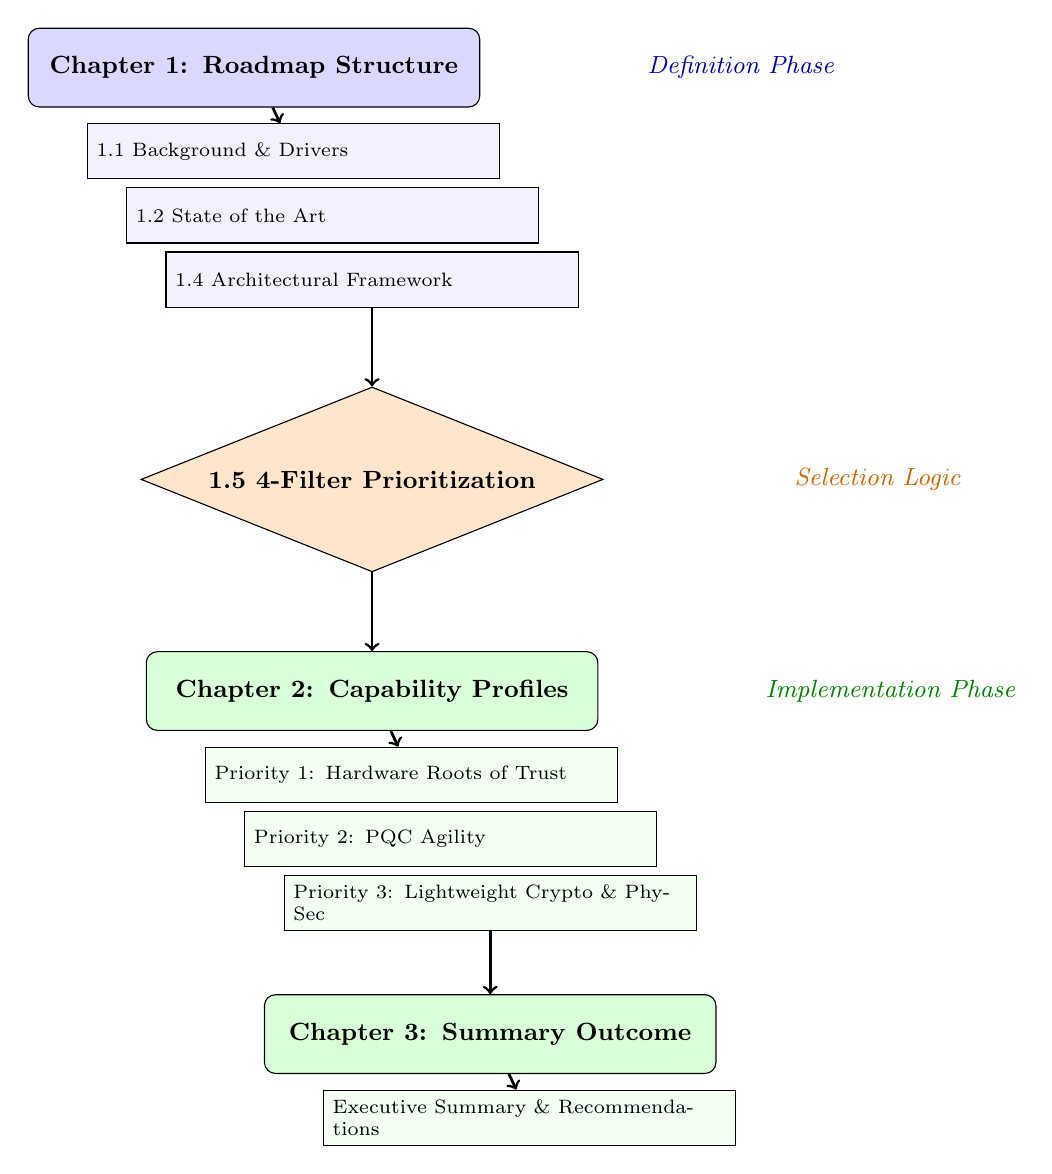
\begin{tikzpicture}[
        node distance=1.2cm and 0.5cm,
        chapter/.style={draw, fill=blue!15, text width=5.5cm, align=center, minimum height=1cm, font=\small\bfseries, rounded corners},
        section/.style={draw, fill=blue!5, text width=5cm, align=left, minimum height=0.7cm, font=\scriptsize, xshift=0.5cm},
        filter/.style={draw, fill=orange!20, text width=4.5cm, align=center, minimum height=1cm, font=\small\bfseries, diamond, aspect=2.5},
        outcome/.style={draw, fill=green!15, text width=5.5cm, align=center, minimum height=1cm, font=\small\bfseries, rounded corners},
        out_sec/.style={draw, fill=green!5, text width=5cm, align=left, minimum height=0.7cm, font=\scriptsize, xshift=0.5cm}
    ]

    % --- Chapter 1 Structure ---
    \node[chapter] (c1) {Chapter 1: Roadmap Structure};
    \node[section, below=0.2cm of c1] (s11) {1.1 Background \& Drivers};
    \node[section, below=0.1cm of s11] (s12) {1.2 State of the Art};
    \node[section, below=0.1cm of s12] (s14) {1.4 Architectural Framework};
    
    % --- Logical Filter (Prompt Logic) ---
    \node[filter, below=1cm of s14] (logic) {1.5 4-Filter Prioritization};
    
    % --- Chapter 2 Outcomes ---
    \node[outcome, below=1cm of logic] (c2) {Chapter 2: Capability Profiles};
    \node[out_sec, below=0.2cm of c2] (s21) {Priority 1: Hardware Roots of Trust};
    \node[out_sec, below=0.1cm of s21] (s22) {Priority 2: PQC Agility};
    \node[out_sec, below=0.1cm of s22] (s23) {Priority 3: Lightweight Crypto \& PhySec};

    % --- Final Chapter ---
    \node[outcome, below=0.8cm of s23] (c3) {Chapter 3: Summary Outcome};
    \node[out_sec, below=0.2cm of c3] (s31) {Executive Summary \& Recommendations};

    % --- Connections ---
    \draw[->, line width=1pt] (c1) -- (s11);
    \draw[->, line width=1pt] (s14) -- (logic);
    \draw[->, line width=1pt] (logic) -- (c2);
    \draw[->, line width=1pt] (c2) -- (s21);
    \draw[->, line width=1pt] (s23) -- (c3);
    \draw[->, line width=1pt] (c3) -- (s31);

    % Legend/Grouping Labels
    \node[right=2cm of c1, font=\small\itshape, text=blue!70!black] {Definition Phase};
    \node[right=2.3cm of logic, font=\small\itshape, text=orange!80!black] {Selection Logic};
    \node[right=2cm of c2, font=\small\itshape, text=green!50!black] {Implementation Phase};

    \end{tikzpicture}
    \caption{Logical structure of the Roadmap: Mapping Chapter hierarchy to the strategic selection process.}
    \label{fig:chapter_hierarchy_roadmap}
\end{figure}


\chapter{Structure and main components of the Roadmap}
\noindent\textbf{Topic:} Cybersecurity for the Cognitive Computing Continuum\\
\textbf{Destinations:}
\begin{itemize}
    \item \textbf{Primary:} 4. A secure, sovereign European computing continuum infrastructure.
    \item \textbf{Secondary:} 6. European leadership in emerging disruptive computing paradigms.
\end{itemize}

\section{Background \& Driving Factors}
\begin{itemize}
    \item \textbf{Decentralization Risk:} The paradigm shift from the centralized Cloud to a distributed Cloud-Edge-IoT continuum radically expands the attack surface. This creates environments that are often ``too many, too diverse, and too dispersed''  to secure with traditional perimeter defenses.
    \item \textbf{Physical Exposure:} Edge nodes and far-edge IoT devices frequently operate in the field. Unlike hyperscaler data centers, they lack strict physical and environmental security controls, making them highly vulnerable to tampering.
    \item \textbf{Regulatory Pressure:} There is an immediate, complex need to operationalize the NIS2 Directive \cite{nis2}, the Cyber Resilience Act (CRA) \cite{cra}, and the AI Act \cite{aiact} across a highly fragmented technological ecosystem to ensure compliance and market access.
    \item \textbf{Digital Sovereignty:} Europe must urgently reduce its systemic reliance on non-EU technology providers. Doing so will mitigate extra-territorial data access risks and avoid geopolitical vendor lock-in, ensuring independent control over critical infrastructure.
\end{itemize}

\section{Europe in Relation to the State of the Art}
\textbf{Comparison vs. Hyperscalers:}
\begin{itemize}
    \item \textbf{EU Strengths:} Europe leads globally in Trust, Privacy-by-Design, proactive regulation (GDPR, Data Act, AI Act), and rigorous, standardized certification frameworks (e.g., EUCS \cite{eucs}).
    \item \textbf{EU Gaps:} The European market suffers from a lack of unified, hyper-scale security orchestration. Furthermore, there is a critical dependency on non-EU hardware (secure silicon) and highly fragmented threat intelligence sharing among member states.
\end{itemize}
\textbf{Strategic Goal:} To definitively transition the European computing continuum from a state of ``reactive, siloed security''  to an advanced architecture defined by ``autonomous, federated, and certified Security-by-Design.'' 

\section{Strategic Preamble}
\begin{itemize}
    \item \textbf{Context:} This section defines the architectural guardrails required to secure the Cloud-Edge-IoT Continuum. It moves beyond traditional ``perimeter security''  toward a model of Cyber-Resilience---where systems are engineered to proactively anticipate, withstand, recover from, and adapt to attacks while maintaining strict Digital Sovereignty.
    \item \textbf{Approach:} To provide actionable, risk-aware Research \& Innovation (R\&I) priorities, the strategy is organized into a two-part framework:
    \begin{itemize}
        \item \textbf{Capability Profiles (Qualitative):} A deep-dive 7-dimensional analysis defining exactly what needs to be built.
        \item \textbf{Progression Matrix (Quantitative \& Strategic):} A structured timeline tracking the evolution of capabilities through their Operational Deployment Phases and their trajectory toward Strategic Sovereignty.
    \end{itemize}
\end{itemize}

\section{The Core Capability Dimensions (Architectural Framework)}
As it is illustrated in Figure~\ref{fig:security_framework_verticals_boxes}, the roadmap is structured across a cohesive architectural framework that spans four continuum environments (HPC, Cloud, Edge, Devices). The capabilities are organized into Six Security Layers (The Vertical Stack) and Four Transversal Cross-Layers (The Horizontal Enablers).

\subsection*{Part A: The Security Layers (Vertical Stack)}
These layers define the specific technical security controls implemented across the computing infrastructure.

\subsubsection*{Layer 1: Hardware-Centric Security}
\textbf{1.1 Hardware Roots of Trust:} Cryptographically verifiable supply chain trust (e.g., TPM attestation, secure enclaves) ensures physical device integrity. Success depends on driving European open-hardware designs (e.g., RISC-V) toward \textbf{EUCC 'High' assurance level certification} \cite{eucc} to mathematically guarantee resistance against state-level physical tampering and side-channel attacks at the vulnerable far-edge.

\textbf{1.2 Physical-Layer (PHY) Threat Detection \& Fingerprinting:} Exploiting intrinsic wireless channel characteristics, such as Channel State Information (CSI), Carrier Frequency Offset (CFO), and Received Signal Strength Indicator (RSSI). That is to establish real-time, keyless device authentication and anomaly detection at the lowest layer of the stack. This provides a hardware-anchored security primitive that is resilient even when upper-layer cryptographic processing is compromised or infeasible.

\subsubsection*{Layer 2: Software-Centric Security (Middleware/OS)}
\textbf{2.1 OS \& Middleware Hardening:} Securing hypervisors, container runtimes, and distributed operating systems is critical for isolation. This involves hardening KVM/QEMU and supporting sovereign, lightweight Linux distributions optimized for edge resource constraints, ensuring a reduced attack surface for the cognitive continuum.

\textbf{2.2 Secure OTA Patch \& Update Management:} Edge nodes deployed in the field---smart grids, O-RAN radios, industrial gateways---require cryptographically verified, failure-resilient over-the-air (OTA) update pipelines. A compromised or failed update mechanism can render entire fleets of field-deployed nodes permanently vulnerable, making robust OTA management a critical software-layer capability.

\subsubsection*{Layer 3: Application-Centric Security (Apps/Services)}
\textbf{3.1 Workload Security:} Securing containerized applications, microservices, and serverless functions executing dynamically across multi-provider nodes. This is achieved through hardened service meshes and sidecar proxy architectures that provide mutual TLS and granular traffic inspection without impacting performance.

\textbf{3.2 In-Band Network Telemetry (INT) \& Deep Observability:} Embedding ``smart telemetry'' directly into the data packets traversing containerized workloads and service meshes, providing granular, real-time visibility into network behaviour and performance without requiring out-of-band monitoring infrastructure. This feeds high-fidelity signals to security analytics platforms.

\textbf{3.3 API Security Gateway \& Policy Enforcement:} As containerized AI workloads increasingly communicate through REST/gRPC APIs, a dedicated API security gateway provides a unified enforcement point for authentication tokens, rate limiting, schema validation, and payload inspection---preventing injection attacks and data exfiltration at the application boundary.

\subsubsection*{Layer 4: User \& Orchestration-Centric Security}
\textbf{4.1 Zero-Trust Orchestration:} Seamless policy enforcement across a multi-provider computing continuum requires robust Policy Enforcement Point (PEP) and Policy Decision Point (PDP) architectures. This enables continuous authorization and dynamic access controls that adapt to the context of the request.

\textbf{4.2 Federated Identity \& Access Management (IAM):} Cross-domain identity federation and verifiable credentials for machines, users, and automated workloads. Implementing \textbf{Self-Sovereign Identity (SSI)} principles allows for cryptographically secure, decentralized authentication across heterogeneous cloud-edge domains.

\textbf{4.3 Privileged Access Management (PAM) \& Just-In-Time (JIT) Access:} Lateral movement by attackers frequently exploits over-provisioned standing privileges---the precise vector behind major Advanced Persistent Threat (APT) campaigns. PAM and JIT access controls ensure that elevated privileges are granted only for defined, time-bounded sessions with full auditability, minimizing the blast radius of any credential compromise.

\subsubsection*{Layer 5: Data-Centric Security}
\textbf{5.1 End-to-end Confidential Computing:} Data-in-use security through Trusted Execution Environments (TEEs) spanning the entire Cloud-to-IoT data path. Leveraging TEE abstraction layers and remote attestation ensures that sensitive European data remains encrypted even during processing in non-trusted environments.

\textbf{5.2 Post-Quantum \& Cryptographic Agility:} PQC standardization and hybrid crypto deployment are necessary to secure long-lived data. Priority is placed on \textbf{PQC migration for resource-constrained devices}, ensuring that edge infrastructure is resilient against ``Harvest Now, Decrypt Later'' quantum threats.

\textbf{5.3 Signaling (Data) Security:} Moving beyond best-effort packet forwarding by embedding trust directly into the network signaling architecture. This ensures the integrity and authenticity of control-plane messages, preventing hijacking of routing decisions and network configuration across the distributed continuum.

\textbf{5.4 Distributed Reputation \& Trust Networking:} Implementing a ubiquitous, real-time reputation system built on Distributed Ledger Technology (DLT) and smart contracts. This enables autonomous, evidence-based trust decisions about nodes, services, and data sources across the continuum without reliance on a central authority.

\textbf{5.5 Quantum Key Distribution (QKD) for Critical Links:} While PQC addresses algorithmic quantum-resistance, QKD provides information-theoretically secure key exchange over optical fibre for point-to-point high-value links (government, critical infrastructure backbone). These two technologies are complementary and together form a comprehensive quantum-safe strategy.

\textbf{5.6 Secure Multi-Party Computation (SMPC):} Homomorphic Encryption and TEEs (Layer 5.1) handle confidential computing for single-party workloads. SMPC enables multiple mutually distrusting parties to jointly compute a function over their combined private inputs without revealing those inputs to each other---a critical capability for cross-border analytics and federated AI in regulated sectors.

\subsubsection*{Layer 6: Network Infrastructure \& Perimeter-Centric Security}
\textbf{6.1 Telco-cloud \& O-RAN Security:} Hardening distributed 5G/6G cores and RAN components must align with the \textbf{Smart Networks and Services Joint Undertaking (SNS JU) SRIA} \cite{snsju}. This ensures sovereign control over network slice isolation and virtualized RAN components.

\textbf{6.2 Cross-Sector Physical Resilience \& Safety:} Adapting strict network controls and IT/OT gateway security for high-availability edge environments (e.g., Smart Grids). This guarantees that cyber-breaches in the digital layer do not cascade into physical safety hazards or kinetic damage in critical infrastructure.

\textbf{6.3 Edge-Native Autonomous Guardians:} Hosting lightweight, localized security control functions (Security-as-a-Service aggregators) directly at the far-edge gateways or within Open-RAN Radio Intelligent Controllers (RIC). These autonomous guardian nodes execute real-time threat mitigation without requiring round-trip communication to a centralized cloud-based SOC, dramatically reducing response latency.

\textbf{6.4 Non-Terrestrial Network (NTN) \& Satellite Security:} 6G will natively integrate satellite segments for coverage continuity, backhaul resilience, and emergency operations. These non-terrestrial links introduce distinct threat surfaces---including signal interception and orbital spoofing---requiring dedicated security requirements aligned with 3GPP NTN specifications and the EU Space Programme.

\subsection*{Part B: The Transversal Security Verticals (Cross-Layers)}
These four cross-layers represent continuous, automated processes and governance structures that intersect every layer of the vertical stack.

\subsubsection*{Cross-Layer 1: Automated Security Processes \& Cyber-Resilient AI Lifecycle}
\textbf{CL1.1 Continuous DevSecOps (Shift-Left):} Embedding AI-driven code analysis and automated vulnerability remediation at the earliest stages of the software lifecycle.

\textbf{CL1.2 Model \& Pipeline Integrity (DataBOMs):} Securing AI training pipelines to prevent data poisoning and unauthorized model manipulation at the edge, ensuring the reliability of cognitive decisions across the continuum.

\textbf{CL1.3 Dynamic Supply Chain Verification (Runtime SBOMs):} Moving beyond static software manifests by implementing dynamic Software Bill of Materials (Runtime SBOMs) and ``cryptographic proof of execution'' to continuously verify the integrity of containerized microservices and AI components as they migrate across the multi-provider edge-cloud continuum.

\textbf{CL1.4 Automated Adversarial Testing \& Continuous Purple Teaming:} DevSecOps pipelines focus on code analysis and remediation; the adversarial counterpart provides continuous automated penetration testing, fuzzing (coverage-guided and protocol-level), and purple-team automation that simulates real attacker behaviour against live staging environments, ensuring defenses are validated continuously rather than at periodic intervals.

\subsubsection*{Cross-Layer 2: Dynamic Risk Management \& Operational Cyber Resilience}
\textbf{CL2.1 Automated SOC Operations \& Collaborative Threat Intelligence:} Continuous monitoring, SOC federation across Member States, and automated incident containment, underpinned by legally protected, cross-border threat intelligence sharing ecosystems designed to overcome institutional trust barriers and incentivize active collaboration \cite{concordia}.

\textbf{CL2.2 High-Precision Telemetry and Security Signalling:} Implementing ``smart telemetry'' and cybersecurity-related signalling to feed real-time threat intelligence into analytics platforms without overwhelming network bandwidth---ensuring that visibility does not itself become an attack vector or performance bottleneck.

\textbf{CL2.3 Internet of Behavior (IoB) and Evidence Sharing:} Utilizing cybersecurity and QoS signalling traffic to extract and share behavioral patterns across the infrastructure, establishing an ``Internet of Behavior'' that enables proactive anomaly correlation and evidence-based risk assessment at continental scale.

\textbf{CL2.4 AI-Native Analytics Integration (NWDAF \& LLMSecOps):} Routing cybersecurity signalling traffic and telemetry through centralized analytics hubs powered by AI agents. This creates a live ``nervous system'' for the network, allowing AI agents to continuously monitor for zero-day exploits, analyze encrypted traffic flows, and trigger automated incident responses aligned with NWDAF (Network Data Analytics Function) standards.

\textbf{CL2.5 Cyber Threat Intelligence (CTI) Lifecycle Management:} While CL2.1 and CL2.4 consume and act on threat data, explicit governance of the full CTI lifecycle---collection, processing, analysis, dissemination, and feedback---is required as a prerequisite for the federated SOC vision. A sovereign EU CTI platform must define this governance layer to ensure data quality, legal compliance, and attribution reliability.

\textbf{CL2.6 Deception Technology \& Active Defense (Honeynets, Canaries):} Current detection is passive---telemetry is observed and anomalies flagged. Deception adds an active intelligence-collection dimension by deploying decoy assets (honeypots, honeynets, credential canaries, fake API endpoints) that generate high-fidelity, low-noise alerts when touched, enabling early detection of advanced intrusions and insider threats.

\subsubsection*{Cross-Layer 3: Interoperable Security Mechanisms \& Open-Source Verifiability}
\textbf{CL3.1 Heterogeneous Interoperability \& Simpl Integration:} Secure communication and data exchange across disparate systems, edge nodes, and proprietary domains. This includes mandatory alignment with and integration into the Simpl open-source smart middleware \cite{cloud_edge_roadmap} to ensure secure, federated access across Common European Data Spaces.

\textbf{CL3.2 Neutral Host and Multi-Tenant Isolation:} As the ecosystem shifts toward infrastructure sharing and Neutral Host models spanning wireless, optical, and cloud domains, robust isolation between tenants is critical. Security architectures must enforce Zero-Trust edge operations across different network partitions to prevent cross-tenant data leakage and privilege escalation.

\textbf{CL3.3 Pan-European NaaS Federation and Cross-Border Edge Roaming:} Establishing standardized interfaces and harmonized Network APIs (e.g., leveraging CAMARA) to interconnect the fragmented edge clouds of different European telecom operators into a unified Network-as-a-Service (NaaS) platform---enabling a ``Schengen for Cloud/AI'' where compute workloads can roam seamlessly across borders.

\textbf{CL3.4 Semantic Security Interoperability (Common Ontologies \& Data Models):} Federated SOCs and shared threat intelligence only function if participating organisations share a common semantic understanding of security events, asset taxonomies, and risk classifications. Standardized ontologies (e.g., aligned with STIX/TAXII and MITRE ATT\&CK) are a prerequisite for meaningful cross-border correlation.

\textbf{CL3.5 Cyber Range \& Digital Twin Federation for Security Validation:} Before deploying cross-border federated security configurations into production, they must be validated in high-fidelity simulation environments. ENISA already coordinates national cyber range inventories; this cross-layer would federate them into a shared EU-wide infrastructure aligned with the Cyber Solidarity Act's testing provisions.

\subsubsection*{Cross-Layer 4: Compliance-by-Design, Agile Governance \& Automated Assurance}
\textbf{CL4.1 Post-Quantum Readiness \& Zero-Trust Architectures (ZTA):} Moving beyond traditional perimeter-based defenses by embedding continuous, AI-driven Zero-Trust verification and micro-segmentation natively into the cloud-edge infrastructure, combined with a systematic migration roadmap to post-quantum cryptographic primitives across all layers.

\textbf{CL4.2 Continuous Automated Certification:} Replacing ``point-in-time'' PDF certificates with real-time, telemetry-driven certification tracking for both cloud services (\textbf{EUCS}) and physical ICT edge products (\textbf{EUCC}), ensuring that edge nodes autonomously maintain compliance by integrating mandatory vulnerability handling and cryptographic patch verification directly into their operational lifecycle \cite{eucc}.

\textbf{CL4.3 Multicloud Key Management as a Service (KMaaS):} When AI workloads, data flows, and context flows migrate dynamically across a multi-provider computing continuum, managing cryptographic keys and access policies becomes highly complex. KMaaS provides a provider-agnostic, sovereign key lifecycle management capability that prevents key sprawl and ensures revocation propagates consistently across heterogeneous environments.

\textbf{CL4.4 Privacy-Preserving Federated Computation:} When multiple providers work on the same infrastructure, AI training and inference may require access to datasets stored across different jurisdictions and competitive boundaries. Privacy-preserving techniques (federated learning, differential privacy, SMPC) enable collaborative computation while guaranteeing that raw data never leaves its sovereign jurisdiction.

\textbf{CL4.6 Cyber Risk Quantification \& Board-Level Reporting (CRQ):} Compliance frameworks define what controls to implement. A dedicated cross-layer translates technical security posture into financial and operational risk language for decision-makers---potentially in real-time---enabling boards to make informed, evidence-based investment and risk-acceptance decisions aligned with DORA requirements.

\textbf{CL4.7 AI Trustworthiness \& Algorithmic Accountability:} As AI systems themselves become actors within the security architecture---making autonomous containment decisions, classifying threats, orchestrating responses---the trustworthiness of those AI systems becomes a security-critical concern. This layer defines explainability, auditability, and override mechanisms for AI-driven security functions, ensuring alignment with the EU AI Act for high-risk systems.

\section{The 4-Filter Prioritization Framework}
To ensure the roadmap provides actionable guidance for European R\&I funding (Horizon Europe) and strategic investment, capabilities are prioritized using a structured 4-filter logic. This framework identifies the ``Critical Path''  items that require immediate resource allocation in Phase 1 (0-5 Yrs).

\begin{enumerate}
    \item \textbf{Regulatory Urgency (The ``Must-Do''  Filter):}
    \begin{itemize}
        \item \textbf{Question:} Is this capability strictly required to comply with imminent EU law (NIS2 \cite{nis2}, Cyber Resilience Act \cite{cra}, AI Act \cite{aiact})?
        \item \textbf{Logic:} If failure to achieve this by 2026 results in market exclusion or systemic non-compliance, it is designated as \textbf{Priority \#1}.
    \end{itemize}

    \item \textbf{Foundational Dependency (The ``Blocker''  Filter):}
    \begin{itemize}
        \item \textbf{Question:} Do subsequent security layers depend on this capability existing first?
        \item \textbf{Logic:} Foundational technologies (e.g., Layer 1 Hardware Trust) outrank high-level software orchestration. You cannot secure the user (Layer 4) if the hardware (Layer 1) cannot provide a verifiable anchor.
    \end{itemize}

    \item \textbf{The Sovereignty Cliff (The ``Extinction''  Filter):}
    \begin{itemize}
        \item \textbf{Question:} Does a lack of this tech pose an existential threat to EU sovereignty or systemic resilience?
        \item \textbf{Logic:} This prioritizes areas where the EU currently has 100\% foreign dependency or where a technical breakthrough (e.g., \textit{Q-Day} Quantum threat) would render existing defenses obsolete.
    \end{itemize}

    \item \textbf{Market Feasibility \& Ecosystem (The ``Simpl/SME''  Filter):}
    \begin{itemize}
        \item \textbf{Question:} Does this align with existing EU heavy-investments (e.g., Simpl \cite{cloud_edge_roadmap}) and is it adoptable by SMEs?
        \item \textbf{Logic:} Priority is given to capabilities that act as force-multipliers for existing infrastructure, ensuring economic viability.
    \end{itemize}
\end{enumerate}

\section*{Executive Priorities: The Critical Path (Phase 1)}
Applying the 4-Filter Framework, the following areas are identified as immediate strategic priorities for the 2025-2030 funding cycle:
\begin{itemize}
    \item \textbf{Priority 1:} Hardware Roots of Trust \& EUCC 'High' Certification (Filters 1, 2, 3).
    \item \textbf{Priority 2:} Post-Quantum Cryptographic (PQC) Agility for Edge/IoT (Filter 3).
    \item \textbf{Priority 3:} Lightweight Cryptography \& Physical-Layer Security (PhySec) for the Extreme Edge (Filters 2, 3).
    \item \textbf{Priority 4:} Security Interoperability via Simpl Middleware (Filter 4).
    \item \textbf{Priority 5:} Supply Chain Verification and Secured Infrastructure (Filters 1, 2).
    \item \textbf{Priority 6:} Cognitive SecOps (LLMSecOps) \& Automated Threat Intelligence (Filters 1, 4).
    \item \textbf{Priority 7:} Pan-European NaaS Federation (``Schengen for Cloud-Edge/AI'') (Filter 4).
    \item \textbf{Priority 8:} Confidential Computing \& Privacy-Preserving AI Pipelines (Filters 1, 3).
    \item \textbf{Priority 9:} Resilient-by-Design Infrastructure \& Autonomous ``Island Mode'' (Filters 1, 2).
    \item \textbf{Priority 10:} Proactive Cyber Threat Management \& Defense against Advanced Persistent Threats (APTs) (Filters 1, 3).
\end{itemize}

\section{The Anatomy of a Roadmap Priority: A 7-Dimensional Analysis}
To ensure the roadmap is actionable, realistic, and aligned with European strategic autonomy, every priority is analyzed holistically through a strict 7-point structural template:

\begin{enumerate}
    \item \textbf{Baseline \& Target Objective (The Trajectory) - Q: Where do we stand today, and what exactly does success look like?}\\
    \textit{Description:} Establishes the starting point of the priority today and defines the ultimate maturity state required by the end of the 15-year roadmap.
    \begin{itemize}
    \item \textbf{Baseline (Where we are):} Grounds the roadmap in reality. It captures the state of the art, current Operational Deployment Phase (ODP), Strategic Sovereignty Level (SSL), industrial capacity, reliance on foreign vendors, and the technical or economic barriers preventing immediate adoption.
    \item \textbf{Target (Where we need to be):} Sets the baseline for EU-funded projects, defining the target ODP and SSL that must be achieved by the end of the roadmap.
\end{itemize}
    
    \item \textbf{Primary Drivers (The ``Push''  Factors) - Q: Why must we prioritize building this capability right now?}\\
    \textit{Description:} Outlines the external pressures---both from the evolving threat landscape and mandatory EU regulations---that make this technological evolution urgent and unavoidable.

    \item \textbf{High Impact Activities - Q: Which specific actions provide the greatest leap in European sovereignty and security?}\\
    \textit{Description:} Highlights the specific, prioritized technical interventions within this broader capability group that will yield the highest strategic return on investment.

    \item \textbf{Catalysts \& Enablers (The ``Pull''  Factors \& EU Support) - Q: What specific EU funding, standards, and ecosystem support do we need?}\\
    \textit{Description:} Identifies the concrete mechanisms, funding vehicles, and regulatory standardizations required from the EU to accelerate market adoption.

    \item \textbf{Disruptors \& Systemic Risks (The Roadblocks) - Q: What structural vulnerabilities, market failures, or adversary breakthroughs could derail us?}\\
    \textit{Description:} Acknowledges that innovation is not linear by identifying severe technical and architectural risks that could actively derail deployment.

    \item \textbf{Failsafe Mechanisms \& Resilience (The Safety Nets) - Q: If this technology is compromised, how does the system survive and gracefully degrade?}\\
    \textit{Description:} The technical core of ``Cyber-Resilience.'' Defines the engineering fallbacks required if a primary capability fails, is breached, or is disrupted.

    \item \textbf{Transversal Meta-Layer (The Policy Alignment) - Q: How does mastering this capability support Europe's goals of sovereignty, sustainability, and trust?}\\
    \textit{Description:} Elevates the technical capability back to the overarching political and societal goals of the European Union.
\end{enumerate}

\section{Progression Matrix: Sequence of Events (X-Axis)}

\begin{itemize}
    \item \textbf{Phase 1: Foundation \& Compliance (Immediate Implementation):} Focuses on state-of-practice deployments, bridging immediate capability gaps, and addressing urgent regulatory obligations (NIS2, CRA).
    \item \textbf{Phase 2: Federation \& Standardization (Scaling \& Harmonization):} Focuses on deploying emerging technologies, establishing harmonized governance frameworks, and managing critical transition periods.
    \item \textbf{Phase 3: Autonomy \& Leadership (Sovereign Innovation):} Focuses on highly speculative but structured foresight, including defense against quantum-capable adversaries and the achievement of fully sovereign, autonomous cloud-edge ecosystems.
\end{itemize}

\subsection*{Matrix Cell Content Definition (Measuring Progression)}
\begin{itemize}
    \item \textbf{Operational Deployment Phase (ODP):} Tracks the market reality and integration status (e.g., \textit{Applied R\&D $\rightarrow$ Fragmented Piloting $\rightarrow$ Standardized Integration $\rightarrow$ Ubiquitous Operation}).
    \item \textbf{Strategic Sovereignty Level (SSL):} Tracks European strategic autonomy and reliance on foreign vendors (e.g., \textit{High Foreign Dependency $\rightarrow$ Emerging EU Ecosystem $\rightarrow$ Full Sovereign Autonomy}).
    \item \textbf{Operational State:} A concise snapshot characterizing the reality on the ground during this phase.
    \item \textbf{Critical Enabler:} The single most critical regulation, standard, or European R\&I breakthrough unlocking the transition to the next phase.
\end{itemize}

\newpage
% =========================================================================
% CHAPTER 1: INSTRUCTIONS
% =========================================================================
\chapter{Instructions for Using This Roadmap Framework}

\subsection*{Purpose of This Document}
This roadmap provides a structured methodology for European policymakers, research organizations, and industry stakeholders to:
\begin{itemize}
    \item Identify and prioritize cybersecurity R\&I investments for the Cloud-Edge-IoT continuum
    \item Track capability maturity using objective Operational Deployment Phase (ODP) and Strategic Sovereignty Level (SSL) metrics
    \item Align Horizon Europe funding with strategic autonomy goals and regulatory compliance requirements
    \item Ensure coordinated implementation across Member States and European initiatives (ECCC, Digital Europe Programme, EU Chips Act)
\end{itemize}

\subsection*{Target Audiences}
\begin{description}
    \item[European Commission \& Funding Bodies:] Use the 4-Filter Prioritization Framework to allocate Horizon Europe, Digital Europe Programme, and ECCC funding to capabilities with the highest strategic impact.
    
    \item[National Cybersecurity Agencies:] Leverage the progression matrices to coordinate national R\&I investments with EU-wide timelines and ensure interoperability across Member States.
    
    \item[Research Consortia \& Industry:] Utilize the 7-Dimensional Analysis template to structure project proposals, clearly articulating baseline, target, drivers, risks, and alignment with European strategic goals.
    
    \item[Standardization Bodies (CEN/CENELEC, ETSI):] Reference the architectural framework and MIMs to develop harmonized standards for secure, interoperable computing continuum infrastructure.
\end{description}

\subsection*{How to Navigate This Document}
\begin{enumerate}
    \item \textbf{Start with Section 1-3:} Understand the threat landscape, regulatory drivers, and strategic context for securing the European computing continuum.
    \item \textbf{Review Section 4:} Familiarize yourself with the 6 Security Layers and 4 Cross-Layers comprising the architectural framework.
    \item \textbf{Apply Section 5:} Use the 4-Filter Prioritization Framework to assess which capabilities are critical for your specific context.
    \item \textbf{Study Section 6-7:} Understand the 7-Dimensional Analysis methodology and ODP/SSL progression metrics before designing projects or policies.
    \item \textbf{Reference Section 9 (Priorities 1-10):} Use the detailed capability profiles as templates for structuring additional priorities relevant to your domain.
    \item \textbf{Implement Section 10:} Actionable strategic recommendations for Phase 1 (2025-2030) provide concrete next steps.
\end{enumerate}

\subsection*{Key Principles}
\begin{itemize}
    \item \textbf{Evidence-Based Prioritization:} All priorities must pass the 4-Filter Framework.
    \item \textbf{Sovereignty-First Design:} Investments should systematically reduce foreign dependencies (measured via SSL metrics) while building European industrial capacity.
    \item \textbf{Compliance-by-Design:} All R\&I outputs must align with or anticipate NIS2, CRA, AI Act, and Data Act requirements.
    \item \textbf{Federated Interoperability:} Solutions must prioritize standardization and open architectures over proprietary, siloed approaches.
    \item \textbf{Measurable Progression:} Avoid subjective TRL assessments; instead, use objective ODP and SSL metrics with clear phase transition criteria.
\end{itemize}

\newpage
% =========================================================================
% CHAPTER 2: PROMPT
% =========================================================================
\section{Master Prompt for Generating Capability Profiles}

\subsection*{Context for Content Generation}
You are an expert EU Cybersecurity Policy Strategist and Technical Architect. Your task is to populate capability profiles for the European Cloud-Edge-IoT Cybersecurity Roadmap using the structured framework defined in this document. Each capability profile must be rigorously aligned with European strategic autonomy goals, regulatory requirements, and the specific needs of the distributed computing continuum.

\subsection*{Input Requirements}
Before generating a capability profile, ensure you have:
\begin{itemize}
    \item \textbf{Capability Name:} Clear, concise identifier
    \item \textbf{Architectural Placement:} Which Layer(s) or Cross-Layer(s) does this capability belong to?
    \item \textbf{Priority Justification:} Which filters from the 4-Filter Framework does this capability satisfy?
    \item \textbf{Contextual Scope:} Is this capability specific to HPC, Cloud, Edge, or Devices?
\end{itemize}

\subsection*{Generation Template: 7-Dimensional Analysis}

\subsubsection*{Dimension 1: Baseline \& Target Objective}
\begin{itemize}
    \item \textbf{Baseline (Current State):} Describe the state of the art in Europe as of 2025-2026. Include current ODP/SSL level, technical/economic barriers, and vendor lock-in issues.
    \item \textbf{Target (Desired State by 2040):} Define success with target ODP/SSL and measurable technical outcomes.
\end{itemize}

\subsubsection*{Dimension 2: Primary Drivers}
\begin{itemize}
    \item \textbf{Threat Drivers:} What adversarial capabilities or attack vectors make this urgent?
    \item \textbf{Regulatory Drivers:} Which EU laws mandate or incentivize this capability?
\end{itemize}

\subsubsection*{Dimension 3: High Impact Activities}
List 3-5 specific technical interventions that will yield the greatest strategic ROI.

\subsubsection*{Dimension 4: Catalysts \& Enablers}
\begin{itemize}
    \item \textbf{Funding Alignment:} Horizon Europe clusters, Digital Europe Programme, ECCC work packages.
    \item \textbf{Standardization:} CEN/CENELEC, ETSI, or ISO standards required.
    \item \textbf{Ecosystem Enablers:} Pilot infrastructure, industry partnerships, SME support schemes.
\end{itemize}

\subsubsection*{Dimension 5: Disruptors \& Systemic Risks}
\begin{itemize}
    \item \textbf{Technical Cliffs:} Q-Day, TEE side-channel breakthroughs, etc.
    \item \textbf{Market \& Supply Chain:} Fabrication delays, vendor resistance, monopolization.
    \item \textbf{Geopolitical:} Export controls, extra-territorial jurisdiction conflicts.
\end{itemize}

\subsubsection*{Dimension 6: Failsafe Mechanisms \& Resilience}
\begin{itemize}
    \item \textbf{Redundancy:} Hybrid approaches during transition periods.
    \item \textbf{Graceful Degradation:} Continued operation in a compromised state.
    \item \textbf{Autonomous Isolation:} Automated quarantine protocols.
    \item \textbf{Implementation Diversity:} Avoiding monocultures.
\end{itemize}

\subsubsection*{Dimension 7: Transversal Meta-Layer}
\begin{itemize}
    \item \textbf{Sovereignty \& Autonomy:} Reduction of extra-territorial dependencies.
    \item \textbf{Trust \& Ethics:} GDPR, Privacy-by-Design, algorithmic transparency.
    \item \textbf{Sustainability (Green IT):} Energy efficiency, e-waste reduction.
\end{itemize}

\subsection*{Mandatory Integration Points}
All generated profiles MUST reference:
\begin{itemize}
    \item \textbf{Simpl Middleware:} For cross-provider interoperability or Data Spaces (CL3.1)
    \item \textbf{SNS JU SRIA:} For 5G/6G, network slicing, or telco-cloud (Layer 6.1)
    \item \textbf{EUCS/EUCC:} For certification, compliance automation, or assurance (CL4.2)
    \item \textbf{ECCC Strategic Agenda:} All profiles must align funding recommendations with ECCC priorities
\end{itemize}

\newpage
% =========================================================================
% CHAPTER 3: EXECUTION
% =========================================================================
\section{Execution Roadmap for Implementation}

\subsection*{Phase 1: Foundation \& Compliance (2025-2030)}

\subsubsection*{Year 1-2 (2025-2026): Strategic Alignment \& Pilot Initiation}
\textbf{Policy \& Governance Actions:}
\begin{itemize}
    \item Establish inter-DG coordination mechanism (DG CONNECT, DG CNECT, ECCC) for unified cybersecurity investment strategy
    \item Finalize and publish EU-wide PQC migration guidelines (ENISA lead)
    \item Launch Simpl Governance Board with security workstream mandate
    \item Issue Horizon Europe calls explicitly aligned with Priority 1-5 (Hardware RoT, PQC, PhySec, Simpl, Supply Chain)
\end{itemize}

\textbf{R\&I \& Technology Actions:}
\begin{itemize}
    \item Fund 3-5 RISC-V secure element pilot projects targeting EUCC 'High' certification
    \item Initiate PQC optimization research for 8/16-bit microcontrollers (embedded systems focus)
    \item Deploy Simpl security MIM pilots in 2-3 Data Spaces (e.g., Manufacturing, Health)
    \item Establish federated Cyber Range infrastructure for cross-border SOC training
    \item Launch Runtime SBOM and Digital Product Passport pilot programmes for supply chain transparency
\end{itemize}

\textbf{Success Metrics:}
\begin{itemize}
    \item At least 50M EUR allocated to sovereign secure silicon R\&D
    \item ENISA PQC guidelines published and adopted by 5+ Member States
    \item 2+ Common Data Spaces operationally testing Simpl security modules
\end{itemize}

\subsubsection*{Year 3-4 (2027-2028): Standardization \& Scale-Up}
\textbf{Policy \& Governance Actions:}
\begin{itemize}
    \item Enforce CRA compliance verification for all new IoT/edge products entering EU market
    \item Publish CEN/CENELEC standards for security MIMs and crypto-agility frameworks
    \item Establish continuous certification pilot programs for EUCS/EUCC
    \item Launch EU Chips Act secure silicon fabrication pilot lines
\end{itemize}

\textbf{R\&I \& Technology Actions:}
\begin{itemize}
    \item Transition RISC-V secure elements from TRL 6-7 to industrial production (TRL 8-9)
    \item Deploy hybrid PQC schemes in critical infrastructure (energy grids, financial systems)
    \item Scale Simpl-based security across 50\%+ of active Common Data Spaces
    \item Operationalize automated SOC federation with cross-border threat intelligence sharing
    \item Deploy LLMSecOps copilots in national CERT/SOC environments
\end{itemize}

\subsubsection*{Year 5 (2029-2030): Market Penetration \& Assessment}
\begin{itemize}
    \item Conduct comprehensive Phase 1 evaluation against 2030 success metrics
    \item Achieve 30\%+ market share for EU secure silicon in critical edge infrastructure
    \item Complete cryptographic inventory of 80\%+ legacy OT/IoT systems
    \item Demonstrate fully automated, real-time EUCS/EUCC certification tracking
\end{itemize}

\subsection*{Phase 2: Federation \& Standardization (2030-2035)}
\begin{itemize}
    \item \textbf{Quantum-Resilient Continuum:} Complete PQC migration for all critical infrastructure
    \item \textbf{Autonomous Security Orchestration:} Deploy AI-driven zero-trust policy enforcement
    \item \textbf{European Certification Fabric:} Ubiquitous continuous certification
    \item \textbf{Sovereign Supply Chains:} Achieve 60\%+ EU market share for secure silicon
    \item \textbf{Federated SOC Operations:} Pan-European CTI sharing fully operational
\end{itemize}

\subsection*{Phase 3: Autonomy \& Leadership (2035-2040)}
\begin{itemize}
    \item \textbf{Full Sovereign Autonomy (SSL):} EU-designed security components dominate European market
    \item \textbf{Ubiquitous Operation (ODP):} Security-by-Design is the default
    \item \textbf{Export Leadership:} European cybersecurity standards become global reference implementations
    \item \textbf{AI-Native Defense:} Swarm-based autonomous threat management across the continuum
\end{itemize}

\newpage
% =========================================================================
% CAPABILITY PROFILES
% =========================================================================
\section{Capability Profiles \& Progression Matrices}

% -----------------------------------------------------------------------
\subsection*{Priority 1: Hardware Roots of Trust \& EUCC 'High' Certification}
% -----------------------------------------------------------------------

\begin{enumerate}
\item \textbf{Baseline \& Target Objective:}
\textit{Baseline:} High foreign dependency on proprietary Trusted Platform Modules (TPMs) and secure elements. Far-edge devices lack standardized hardware anchors.
\textit{Target:} Ubiquitous deployment of EU-designed, open-source (RISC-V) secure enclaves certified at \textbf{EUCC 'High' assurance}, providing a mathematically verifiable foundation for the entire continuum.

\item \textbf{Primary Drivers:} 
\textit{Threat:} State-level physical tampering and side-channel attacks on decentralized edge nodes. 
\textit{Regulatory:} Mandatory hardware security requirements under the \textbf{Cyber Resilience Act (CRA)} and certified anchors for \textbf{NIS2} critical infrastructure.

\item \textbf{High Impact Activities:} 
Development of sovereign European Secure Elements based on RISC-V; automated hardware-level remote attestation protocols for large-scale edge fleets; EU-level standard toolset developed and maintained by the European Commission; SME support for certification and compliance testing; security-based sensor research for future deployment.

\item \textbf{Catalysts \& Enablers:} 
\textbf{EU Chips Act} pilot lines for secure silicon; \textbf{ECCC Strategic Agenda} funding for open-hardware security; alignment with CEN/CENELEC hardware security standards.

\item \textbf{Disruptors \& Systemic Risks:} 
Supply chain bottlenecks for EU-based fabrication; breakthroughs in physical side-channel analysis that bypass current cryptographic enclaves.

\item \textbf{Failsafe Mechanisms \& Resilience:} 
``Defense-in-depth'' where software-based isolation (TEEs) acts as a secondary layer if a hardware enclave is compromised; autonomous node isolation and distributed attestation if hardware integrity is lost.

\item \textbf{Transversal Meta-Layer:} 
\textit{Sovereignty:} Eliminates ``black-box'' hardware dependencies on non-EU vendors. \textit{Sustainability:} Energy-efficient secure silicon designs reducing the carbon footprint of cryptographic operations at the far-edge.

\end{enumerate}

\vspace{0.3cm}
\noindent\textbf{Progression Matrix: Hardware Roots of Trust \& EUCC 'High'}
\vspace{0.2cm}

\noindent\resizebox{\textwidth}{!}{%
\begin{tabular}{|p{3cm}|p{4.5cm}|p{4.5cm}|p{4.5cm}|}
\hline
\textbf{Metric} & \textbf{Phase 1: Foundation \& Compliance (0-5 Yrs)} & \textbf{Phase 2: Federation \& Standardization (5-10 Yrs)} & \textbf{Phase 3: Autonomy \& Leadership (10-15 Yrs)} \\ \hline
\textbf{ODP} & Fragmented Piloting & Standardized Integration & Ubiquitous Operation \\ \hline
\textbf{SSL} & High Foreign Dependency & Emerging EU Ecosystem & Full Sovereign Autonomy \\ \hline
\textbf{Operational State} & Cloud-based TPMs common; Edge nodes lack hardware trust; RISC-V pilots begin; CRA compliance starts. & Standardized EU-made secure elements in critical infra; Automated attestation at scale. & Sovereign hardware trust embedded by default in all EU ICT products from IoT to HPC. \\ \hline
\textbf{Critical Enabler} & \textbf{Cyber Resilience Act (CRA)} enforcement & \textbf{EUCC 'High'} certification of EU-based secure elements & Maturity of \textbf{EU Chips Act} sovereign fabrication lines \\ \hline
\end{tabular}%
}

% -----------------------------------------------------------------------
\subsection*{Priority 2: Post-Quantum Cryptographic (PQC) Agility for Edge/IoT}
% -----------------------------------------------------------------------

\begin{enumerate}
\item \textbf{Baseline \& Target Objective:}
\textit{Baseline:} Current IoT and edge infrastructure predominantly relies on classical cryptography (RSA, ECC) vulnerable to future quantum computers. Limited awareness and no systematic migration path for resource-constrained devices.
\textit{Target:} A ``Quantum-Native'' continuum where all critical edge/IoT infrastructure has migrated to hybrid or full Post-Quantum Cryptography, with automated crypto-agility enabling seamless algorithm updates without hardware replacement.

\item \textbf{Primary Drivers:} 
\textit{Threat:} The \textbf{Q-Day} threat and ``Harvest Now, Decrypt Later'' strategies targeting sensitive long-lived data.
\textit{Regulatory:} Emerging ENISA guidelines and future EU mandates requiring PQC readiness for critical infrastructure under NIS2.

\item \textbf{High Impact Activities:} 
Optimization of NIST-standardized PQC algorithms for 8/16-bit microcontrollers; development of crypto-agility middleware for OTA algorithm updates; automated cryptographic inventory and migration tools for legacy IoT deployments; 3GPP specifications alignment for quantum key distribution (QKD) in cellular systems.

\item \textbf{Catalysts \& Enablers:} 
\textbf{NIST PQC standardization finalization}; \textbf{ETSI} quantum-safe cryptography standards; \textbf{ENISA PQC guidelines}; \textbf{ECCC Strategic Agenda} funding; EU Chips Act for PQC-native silicon development.

\item \textbf{Disruptors \& Systemic Risks:} 
Early arrival of CRQC before migration is complete; performance overhead of PQC algorithms on battery-powered IoT; fragmented standardization; insufficient cryptographic inventory of legacy OT/IoT systems.

\item \textbf{Failsafe Mechanisms \& Resilience:} 
Deployment of hybrid cryptographic schemes (classical + PQC) during the transition; crypto-agility frameworks allowing rapid algorithm switching if vulnerabilities are discovered; diversification of PQC algorithm families to avoid single-point cryptanalytic failures.

\item \textbf{Transversal Meta-Layer:} 
\textit{Sovereignty:} Protection of Europe's long-term industrial and governmental secrets from future quantum decryption. \textit{Sustainability:} Energy-efficient, lightweight PQC implementations reducing the carbon footprint of security (Green IT).

\end{enumerate}

\vspace{0.3cm}
\noindent\textbf{Progression Matrix: PQC Agility for Edge/IoT}
\vspace{0.2cm}

\noindent\resizebox{\textwidth}{!}{%
\begin{tabular}{|p{3cm}|p{4.5cm}|p{4.5cm}|p{4.5cm}|}
\hline
\textbf{Metric} & \textbf{Phase 1: Foundation \& Compliance (0-5 Yrs)} & \textbf{Phase 2: Federation \& Standardization (5-10 Yrs)} & \textbf{Phase 3: Autonomy \& Leadership (10-15 Yrs)} \\ \hline
\textbf{ODP} & Applied R\&D & Fragmented Piloting & Ubiquitous Operation \\ \hline
\textbf{SSL} & High Foreign Dependency & Emerging EU Ecosystem & Full Sovereign Autonomy \\ \hline
\textbf{Operational State} & NIST algorithm selection; software-based PQC pilots in cloud environments; research on lightweight implementations. & Hybrid (classical + PQC) schemes in Industrial IoT and critical edge infrastructure; EU-developed crypto-agility middleware. & Fully quantum-resilient continuum with PQC embedded in all devices; automated crypto-agility across Cloud-Edge-IoT. \\ \hline
\textbf{Critical Enabler} & \textbf{ENISA PQC Guidelines} and NIST standardization completion & \textbf{NIST/ETSI} algorithm finalization and EU-wide deployment standards & PQC-native \textbf{RISC-V silicon} and ubiquitous crypto-agility frameworks \\ \hline
\end{tabular}%
}

% -----------------------------------------------------------------------
\subsection*{Priority 3: Lightweight Cryptography \& Physical-Layer Security (PhySec) for the Extreme Edge}
% -----------------------------------------------------------------------

\begin{enumerate}
\item \textbf{Baseline \& Target Objective:}
\textit{Baseline:} Massive IoT and nano-devices cannot support computationally heavy classical asymmetric encryption. Current security approaches are unsuitable for environments requiring 100 devices per m\textsuperscript{3} with 40-year battery lifespans or zero-energy backscatter radios.
\textit{Target:} Move to ultra-lightweight Post-Quantum Cryptography and keyless Physical-Layer Security (PhySec) embedded at the extreme edge, enabling security primitives that operate within severe energy and compute constraints.

\item \textbf{Primary Drivers:} 
\textit{Threat:} The proliferation of massive Machine Type Communication (mMTC) creates an enormous unprotected attack surface; classical cryptography is both computationally infeasible and imminently vulnerable to quantum algorithms at the extreme edge.
\textit{Regulatory:} CRA requirements extend to the smallest connected devices; NIS2 mandates security across the full infrastructure including resource-constrained nodes.

\item \textbf{High Impact Activities:} 
Group-based authentication for large-scale constrained IoT fleets; RF fingerprinting and Channel State Information (CSI)-based device authentication; integration of lightweight PQC into European open-hardware (RISC-V) for smart body-area networks (WBAN); ETSI SmartBAN standardization alignment; research into ``zero-energy'' air interfaces with integrated Integrated Sensing and Communication (ISAC) security.

\item \textbf{Catalysts \& Enablers:} 
NIST lightweight post-quantum cryptography standardization; ETSI SmartBAN standardization; 6G research into RF fingerprinting and channel entropy for native security; Hardware-Software Co-Design for neuromorphic and Processing-in-Memory (PIM) architectures.

\item \textbf{Disruptors \& Systemic Risks:} 
Performance gap between available energy budgets and minimum cryptographic processing requirements; fragmented device ecosystems preventing uniform PhySec adoption; lack of EU-manufactured ultra-constrained secure silicon.

\item \textbf{Failsafe Mechanisms \& Resilience:} 
Dynamic fallback to localized, non-routed trust boundaries leveraging purely physical-layer signatures (RF fingerprinting or channel entropy) to authenticate devices if upper-layer cryptographic processing exceeds the available energy budget or is compromised.

\item \textbf{Transversal Meta-Layer:} 
\textit{Sovereignty:} Sovereign control over the security of the most proliferated and currently most unprotected layer of the computing continuum. \textit{Sustainability:} Zero-energy security primitives are inherently aligned with Green IT objectives and circular economy principles.

\end{enumerate}

\vspace{0.3cm}
\noindent\textbf{Progression Matrix: Lightweight Cryptography \& PhySec for the Extreme Edge}
\vspace{0.2cm}

\noindent\resizebox{\textwidth}{!}{%
\begin{tabular}{|p{3cm}|p{4.5cm}|p{4.5cm}|p{4.5cm}|}
\hline
\textbf{Metric} & \textbf{Phase 1: Foundation \& Compliance (0-5 Yrs)} & \textbf{Phase 2: Federation \& Standardization (5-10 Yrs)} & \textbf{Phase 3: Autonomy \& Leadership (10-15 Yrs)} \\ \hline
\textbf{ODP} & Isolated Lightweight Piloting & Standardized D2D Security Integration & Ubiquitous Zero-Energy Trust \\ \hline
\textbf{SSL} & High Dependency on Legacy/Heavy Algorithms & Emerging EU Lightweight \& PhySec Ecosystem & Full Sovereign Extreme-Edge Cryptography \\ \hline
\textbf{Operational State} & Group-based authentication and early lightweight PQC algorithms tested on resource-constrained IoT; basic RF fingerprinting used for anomaly detection. & Lightweight PQC and PhySec natively embedded in European open-hardware (RISC-V) and smart body-area networks (WBAN). & Battery-less (zero-energy) nodes autonomously execute quantum-resistant authentication and trusted decentralized swarm communications. \\ \hline
\textbf{Critical Enabler} & NIST Lightweight PQC Standards \& Context-Aware IoT Platforms & Hardware-Software Co-Design for Neuromorphic/PIM AI & ``Zero-Energy'' Air Interfaces \& Ubiquitous ISAC (Integrated Sensing and Communication) \\ \hline
\end{tabular}%
}

% -----------------------------------------------------------------------
\subsection*{Priority 4: Security Interoperability via Simpl Middleware}
% -----------------------------------------------------------------------

\begin{enumerate}
\item \textbf{Baseline \& Target Objective:}
\textit{Baseline:} Current European cloud and edge infrastructure is highly fragmented across proprietary vendor silos with incompatible security policies, authentication mechanisms, and data exchange protocols. This fragmentation prevents seamless data flow across Common European Data Spaces and creates vendor lock-in.
\textit{Target:} A unified European ``Trust Fabric'' enabling secure, federated interoperability across heterogeneous cloud and edge providers through mandatory integration with the \textbf{Simpl} open-source smart middleware stack, with standardized security Minimal Interoperability Mechanisms (MIMs).

\item \textbf{Primary Drivers:} 
\textit{Regulatory:} \textbf{Data Act} mandates requiring seamless data portability and interoperability; requirements for Common European Data Spaces to operate across multiple providers; NIS2 requirements for coordinated incident response.
\textit{Market:} Breaking vendor lock-in to enable European SMEs to compete; enabling cross-border data flows while maintaining sovereignty.

\item \textbf{High Impact Activities:} 
Implementation and standardization of security-specific \textbf{MIMs} within the Simpl stack; automated policy translation engines converting provider-specific security policies into common machine-readable format (XACML, OSCAL); federated identity bridges using verifiable credentials; cross-domain security orchestration for unified threat response.

\item \textbf{Catalysts \& Enablers:} 
\textbf{Digital Europe Programme} funding; \textbf{Simpl} open-source stack community and governance; \textbf{Gaia-X} federation services and trust frameworks; ECCC support for security MIM standardization.

\item \textbf{Disruptors \& Systemic Risks:} 
Vendor resistance to open standards; weakest-link security failures in federated systems; complexity of policy translation creating semantic gaps; fragmented national implementations creating ``data islands.''

\item \textbf{Failsafe Mechanisms \& Resilience:} 
Capability to autonomously ``unfederate'' or isolate nodes that fail to meet the shared security baseline; zero-trust architectures where federation does not imply implicit trust; continuous compliance monitoring with automated ejection of non-compliant providers.

\item \textbf{Transversal Meta-Layer:} 
\textit{Sovereignty:} Breaking dependence on non-EU hyperscaler lock-in. \textit{Trust:} Fostering pan-European cross-border trust through transparent, verifiable security mechanisms. \textit{Economic Viability:} Enabling SMEs to participate in Data Spaces without massive infrastructure investments.

\end{enumerate}

\vspace{0.3cm}
\noindent\textbf{Progression Matrix: Security Interoperability via Simpl Middleware}
\vspace{0.2cm}

\noindent\resizebox{\textwidth}{!}{%
\begin{tabular}{|p{3cm}|p{4.5cm}|p{4.5cm}|p{4.5cm}|}
\hline
\textbf{Metric} & \textbf{Phase 1: Foundation \& Compliance (0-5 Yrs)} & \textbf{Phase 2: Federation \& Standardization (5-10 Yrs)} & \textbf{Phase 3: Autonomy \& Leadership (10-15 Yrs)} \\ \hline
\textbf{ODP} & Fragmented Piloting & Standardized Integration & Ubiquitous Operation \\ \hline
\textbf{SSL} & Emerging EU Ecosystem & Full Sovereign Autonomy & Full Sovereign Autonomy \\ \hline
\textbf{Operational State} & Initial Simpl security pilots in select Data Spaces; manual policy coordination; proof-of-concept MIM implementations. & Automated policy translation via standardized MIMs; Simpl-based security in majority of Common Data Spaces; cross-border federated SOC operations. & Fully automated, provider-agnostic European trust fabric; real-time security orchestration across the continuum; zero-trust federation by default. \\ \hline
\textbf{Critical Enabler} & \textbf{Simpl-Open} official launch and initial MIM definitions & Security \textbf{MIMs} adoption as CEN/CENELEC standards & \textbf{EU Cloud Rulebook} maturity and Data Act full enforcement \\ \hline
\end{tabular}%
}

% -----------------------------------------------------------------------
\subsection*{Priority 5: Supply Chain Verification and Secured Infrastructure}
% -----------------------------------------------------------------------

\begin{enumerate}
\item \textbf{Baseline \& Target Objective:}
\textit{Baseline:} Supply chain tracking is static, opaque, and fragmented. The disaggregation of telco clouds (e.g., Open RAN) introduces extreme complexity by mixing software and hardware from multiple vendors. SMEs lack resources to meet CRA and NIS2 supply chain compliance requirements.
\textit{Target:} Move to continuously verified ecosystems utilizing Runtime Software Bill of Materials (SBOMs), Digital Product Passports (DPP), and automated certification across multi-vendor deployments, with full supply chain transparency and sovereign control.

\item \textbf{Primary Drivers:} 
\textit{Threat:} Sophisticated supply chain attacks (e.g., SolarWinds-style compromises) targeting the disaggregated Open RAN and cloud-edge ecosystem; hidden backdoors in non-EU hardware and firmware.
\textit{Regulatory:} Strict legal mandates from the \textbf{Cyber Resilience Act (CRA)} and \textbf{NIS2 Directive} demanding robust supply chain risk management; Digital Product Passport (DPP) initiatives for traceability.

\item \textbf{High Impact Activities:} 
Review and mapping of hardware, OS, and software supply chain vulnerabilities; SME engagement prioritized---ensuring one-size-fits-all approaches are avoided and SMEs can enable new technology integration (e.g., NXP ecosystems); Dynamic Runtime SBOMs tracking active component states; Digital Product Passports for end-to-end traceability; Zero-Knowledge Proofs (ZKPs) for IP-protected component verification.

\item \textbf{Catalysts \& Enablers:} 
Digital Product Passport (DPP) initiatives; European financial support for SME security upskilling; ECCC strategic funding for supply chain security tooling; Pan-European threat intelligence sharing for supply chain indicators of compromise.

\item \textbf{Disruptors \& Systemic Risks:} 
Extreme complexity of multi-vendor Open RAN supply chains; geopolitical dependencies on non-EU component manufacturers; SMEs being priced out of compliance; lack of standardized machine-readable supply chain attestation formats.

\item \textbf{Failsafe Mechanisms \& Resilience:} 
Graceful isolation of unverified or high-risk components into quarantined network slices until cryptographic proofs of execution can validate their integrity; automated blocking of unverified components in production deployments.

\item \textbf{Transversal Meta-Layer:} 
\textit{Sovereignty:} Reducing systemic dependency on non-EU hardware and software supply chains. \textit{Trust:} Providing verifiable, transparent provenance for all components in the European computing continuum. \textit{Economic:} Protecting EU industrial IP through privacy-preserving verification mechanisms.

\end{enumerate}

\vspace{0.3cm}
\noindent\textbf{Progression Matrix: Supply Chain Verification and Secured Infrastructure}
\vspace{0.2cm}

\noindent\resizebox{\textwidth}{!}{%
\begin{tabular}{|p{3cm}|p{4.5cm}|p{4.5cm}|p{4.5cm}|}
\hline
\textbf{Metric} & \textbf{Phase 1: Foundation \& Compliance (0-5 Yrs)} & \textbf{Phase 2: Federation \& Standardization (5-10 Yrs)} & \textbf{Phase 3: Autonomy \& Leadership (10-15 Yrs)} \\ \hline
\textbf{ODP} & Full Supply Chain Disclosure & Partial Restriction Process & Full Restriction Process \\ \hline
\textbf{SSL} & High Reliance on Fragmented, Non-EU Supply Chain Auditing & Emerging EU Supply Chain Tracking Frameworks (DPP) & Full Sovereign Control and Supply Chain Transparency \\ \hline
\textbf{Operational State} & Review of hardware, OS, and software supply chain vulnerabilities; initial Runtime SBOM pilots; CRA compliance mapping begins. & Ensuring certification of critical supply chain hardware, OS, and software; DPP frameworks operational; SME compliance pathways established. & Fully certified supply chain actively blocking unverified components; ZKPs enable IP-protected verification at continental scale. \\ \hline
\textbf{Critical Enabler} & \textbf{CRA} supply chain requirements enforcement; SME engagement programmes & Dynamic Runtime SBOMs and \textbf{Digital Product Passports} & Zero-Knowledge Proofs (ZKPs) \& Pan-European Threat Intel sharing \\ \hline
\end{tabular}%
}

% -----------------------------------------------------------------------
\subsection*{Priority 6: Cognitive SecOps (LLMSecOps) \& Automated Threat Intelligence}
% -----------------------------------------------------------------------

\begin{enumerate}
\item \textbf{Baseline \& Target Objective:}
\textit{Baseline:} Security Operations Centers (SOCs) are predominantly manual, reactive, and siloed. Analyst capacity is far outpaced by the expanding attack surface of 5G/6G and the millions of IoT devices. EU SOCs are heavily reliant on non-EU AI foundation models.
\textit{Target:} Autonomous, AI-driven ``LLMSecOps'' agents distributed across the 6G edge, capable of proactive threat hunting, real-time incident containment, and continuous learning without requiring human intervention for routine responses.

\item \textbf{Primary Drivers:} 
\textit{Threat:} The dual-use nature of AI generating complex offensive threats (APTs, data poisoning, AI-driven exploit generation); the expanding attack surface of 6G and millions of IoT devices overwhelming human-scale SOC operations.
\textit{Regulatory:} EU AI Act compliance for high-risk autonomous security systems; Zero-Touch Network \& Service Management (ZSM) goals; EuroHPC AI Factories as the compute substrate for sovereign AI models.

\item \textbf{High Impact Activities:} 
LLM-assisted human SOC analysts integrated with NWDAF telemetry; edge-native ``Guardian'' nodes executing Zero-Trust reconfigurations autonomously; European sovereign Small Language Models (SLMs) for security classification; swarm-based agentic AI for decentralized threat intelligence; standardized AI Interconnect APIs.

\item \textbf{Catalysts \& Enablers:} 
\textbf{EU AI Act} compliance frameworks for high-risk security AI; \textbf{EuroHPC AI Factories} providing compute for sovereign foundation model training; \textbf{ECCC Strategic Agenda} for LLMSecOps standardization; NWDAF integration with 3GPP standards.

\item \textbf{Disruptors \& Systemic Risks:} 
AI hallucination causing false containment actions disrupting critical services; adversarial attacks on the AI models themselves (prompt injection, model poisoning); regulatory uncertainty around autonomous AI decision-making in security contexts; continued dominance of non-EU foundation models.

\item \textbf{Failsafe Mechanisms \& Resilience:} 
``Shadow-mode'' rollback and human-in-the-loop (RLHF) intervention if autonomous edge agents hallucinate or exhibit unstable control loops; mandatory override mechanisms for all autonomous security decisions affecting critical infrastructure.

\item \textbf{Transversal Meta-Layer:} 
\textit{Sovereignty:} Development of European sovereign edge LLMs and SLMs replacing dependency on US foundation models. \textit{Trust:} Ensuring that AI-driven security decisions are explainable, auditable, and aligned with the EU AI Act for high-risk systems. \textit{Sustainability:} Energy-efficient edge AI inference reducing the carbon footprint of autonomous security operations.

\end{enumerate}

\vspace{0.3cm}
\noindent\textbf{Progression Matrix: Cognitive SecOps (LLMSecOps) \& Automated Threat Intelligence}
\vspace{0.2cm}

\noindent\resizebox{\textwidth}{!}{%
\begin{tabular}{|p{3cm}|p{4.5cm}|p{4.5cm}|p{4.5cm}|}
\hline
\textbf{Metric} & \textbf{Phase 1: Foundation \& Compliance (0-5 Yrs)} & \textbf{Phase 2: Federation \& Standardization (5-10 Yrs)} & \textbf{Phase 3: Autonomy \& Leadership (10-15 Yrs)} \\ \hline
\textbf{ODP} & Siloed AI Copilots & Federated Edge Agents & Ubiquitous AI Immune System \\ \hline
\textbf{SSL} & High Reliance on US Foundation Models & Sovereign European Edge LLMs, SLMs, LCMs & Global Leadership in Trustworthy AI \\ \hline
\textbf{Operational State} & LLMs assist human SOC analysts; NWDAF telemetry routed to centralized AI for anomaly detection. & Edge-native ``Guardian'' nodes autonomously execute Zero-Trust reconfigurations and throttle threats. & Swarm-based agentic AI defends the Edge-Cloud Continuum via decentralized, proactive threat intelligence. \\ \hline
\textbf{Critical Enabler} & \textbf{EU AI Act} enforcement \& EuroHPC AI Factories & Standardized AI Interconnect APIs & Self-Evolving AI Swarm Protocols \\ \hline
\end{tabular}%
}

% -----------------------------------------------------------------------
\subsection*{Priority 7: Pan-European NaaS Federation (``Schengen for Cloud-Edge/AI'')}
% -----------------------------------------------------------------------

\begin{enumerate}
\item \textbf{Baseline \& Target Objective:}
\textit{Baseline:} European telco deployments are fragmented and nation-bound. The lack of a true Digital Single Market prevents European operators from scaling to compete with US and Chinese hyperscalers.
\textit{Target:} A unified, interoperable European Network-as-a-Service (NaaS) platform enabling seamless ``roaming for compute'' across borders, legally operating as a single jurisdiction for data workloads.

\item \textbf{Primary Drivers:} 
\textit{Market:} The ``Sovereignty Cliff''---lack of a true Digital Single Market prevents European operators from achieving scale parity with hyperscalers.
\textit{Regulatory:} Data Act interoperability requirements; IPCEI-CIS mandates for cross-border infrastructure investment; CAMARA API standardization enabling federated network services.

\item \textbf{High Impact Activities:} 
Deployment of harmonized CAMARA APIs; automated compliance negotiation in 5G corridors; ``Data Visa'' mechanisms enabling dynamic cross-border AI model migration; inter-operator East-West security interfaces; development of the ``Schengen for Cloud'' legal framework.

\item \textbf{Catalysts \& Enablers:} 
\textbf{IPCEI-CIS} initial deployments; \textbf{European Alliance for Industrial Data, Edge and Cloud}; \textbf{CAMARA API alliance}; \textbf{Gaia-X} federation services; \textbf{ECCC} for cross-border security standards.

\item \textbf{Disruptors \& Systemic Risks:} 
Conflicting national data sovereignty laws preventing true federation; regulatory arbitrage creating security-weakest-link vulnerabilities at cross-border interfaces; insufficient SLA enforcement mechanisms across operator boundaries.

\item \textbf{Failsafe Mechanisms \& Resilience:} 
Graceful degradation protocols redirect workloads to national infrastructure if cross-border SLAs or compliance APIs fail; bilateral fallback agreements between operator pairs ensuring minimum viable connectivity.

\item \textbf{Transversal Meta-Layer:} 
\textit{Sovereignty:} Enabling European-scale infrastructure that competes with US and Chinese hyperscalers without ceding control to non-EU providers. \textit{Trust:} ``Data Visas'' providing legal clarity on data jurisdiction during cross-border migration. \textit{Economic:} Creating a genuine Digital Single Market that enables European SMEs and operators to compete at continental scale.

\end{enumerate}

\vspace{0.3cm}
\noindent\textbf{Progression Matrix: Pan-European NaaS Federation}
\vspace{0.2cm}

\noindent\resizebox{\textwidth}{!}{%
\begin{tabular}{|p{3cm}|p{4.5cm}|p{4.5cm}|p{4.5cm}|}
\hline
\textbf{Metric} & \textbf{Phase 1: Foundation \& Compliance (0-5 Yrs)} & \textbf{Phase 2: Federation \& Standardization (5-10 Yrs)} & \textbf{Phase 3: Autonomy \& Leadership (10-15 Yrs)} \\ \hline
\textbf{ODP} & Bilateral Interconnection & Federated Edge Roaming & True Digital Single Market \\ \hline
\textbf{SSL} & Hyperscaler Platform Dominance & Pan-European Consortium Competes & European Scale Parity Achieved \\ \hline
\textbf{Operational State} & Harmonized CAMARA APIs deployed; Automated Compliance Negotiators tested in 5G corridors. & ``Data Visas'' enable dynamic cross-border migration of AI models without legal friction. & Single unified computing continuum legally operates as one jurisdiction for data workloads. \\ \hline
\textbf{Critical Enabler} & \textbf{IPCEI-CIS} Initial Deployments & Inter-Operator East-West Interfaces & ``Schengen for Cloud'' Legal Framework \\ \hline
\end{tabular}%
}

% -----------------------------------------------------------------------
\subsection*{Priority 8: Confidential Computing \& Privacy-Preserving AI Pipelines}
% -----------------------------------------------------------------------

\begin{enumerate}
\item \textbf{Baseline \& Target Objective:}
\textit{Baseline:} Basic encryption at-rest and in-transit is standard, but data-in-use remains exposed during processing. Multi-tenant edge nodes and federated AI training create significant insider threat and IP leakage risks.
\textit{Target:} Ubiquitous data-in-use protection via Trusted Execution Environments (TEEs) and Homomorphic Encryption across the full Cloud-to-IoT path, enabling collaborative AI without raw data ever leaving sovereign jurisdictions.

\item \textbf{Primary Drivers:} 
\textit{Threat:} Insider threats in multi-tenant edge nodes; IP exfiltration during federated AI training across competitive organizational boundaries.
\textit{Regulatory:} \textbf{GDPR} stringency for data-in-use; \textbf{EUCS ``High+''} certification requirements mandating confidential computing for sensitive cloud workloads; \textbf{AI Act} requirements for data governance in high-risk AI systems.

\item \textbf{High Impact Activities:} 
TEE deployment on critical cloud nodes for EUCS compliance; sovereign hardware pilots using EU-developed RISC-V TEEs; multi-party privacy-preserving AI pipelines across multi-provider nodes; operationalization of Fully Homomorphic Encryption (FHE) for production analytics workloads.

\item \textbf{Catalysts \& Enablers:} 
\textbf{EUCS} Certification Rollout; \textbf{European Data Spaces} as the deployment vehicle; \textbf{Chips JU} for RISC-V hardware development; \textbf{ECCC} strategic funding for FHE maturation.

\item \textbf{Disruptors \& Systemic Risks:} 
TEE side-channel vulnerabilities rendering current enclave implementations obsolete; FHE performance overhead remaining prohibitive for real-time edge applications; continued dependency on non-EU TEE hardware (Intel SGX, ARM TrustZone).

\item \textbf{Failsafe Mechanisms \& Resilience:} 
Limit processing to local, on-device federated learning nodes (never sharing raw data) if edge TEE integrity cannot be cryptographically verified; multi-TEE implementation diversity to avoid single-vendor hardware vulnerabilities.

\item \textbf{Transversal Meta-Layer:} 
\textit{Sovereignty:} Moving from reliance on foreign hardware TEEs to sovereign RISC-V TEEs. \textit{Trust:} Enabling European citizens and businesses to share data for AI without sacrificing privacy. \textit{Ethics:} Providing the technical foundation for Privacy-by-Design as required by GDPR.

\end{enumerate}

\vspace{0.3cm}
\noindent\textbf{Progression Matrix: Confidential Computing \& Privacy-Preserving AI Pipelines}
\vspace{0.2cm}

\noindent\resizebox{\textwidth}{!}{%
\begin{tabular}{|p{3cm}|p{4.5cm}|p{4.5cm}|p{4.5cm}|}
\hline
\textbf{Metric} & \textbf{Phase 1: Foundation \& Compliance (0-5 Yrs)} & \textbf{Phase 2: Federation \& Standardization (5-10 Yrs)} & \textbf{Phase 3: Autonomy \& Leadership (10-15 Yrs)} \\ \hline
\textbf{ODP} & Isolated Enclaves & Distributed Confidential Cloud & Ubiquitous Confidential Continuum \\ \hline
\textbf{SSL} & High Reliance on Foreign Hardware TPMs & European RISC-V TEEs Emerge & Total Data-in-Use Sovereignty \\ \hline
\textbf{Operational State} & TEEs deployed on critical cloud nodes for EUCS compliance; initial sovereign hardware pilots. & Multi-party privacy-preserving AI pipelines train across multi-provider nodes seamlessly. & Homomorphic encryption operationalized; end-to-end encrypted continuum from IoT to HPC. \\ \hline
\textbf{Critical Enabler} & \textbf{EUCS} Certification Rollout & \textbf{RISC-V} Hardware Scaling & Fully Homomorphic Encryption (FHE) Maturation \\ \hline
\end{tabular}%
}

% -----------------------------------------------------------------------
\subsection*{Priority 9: Resilient-by-Design Infrastructure \& Autonomous ``Island Mode''}
% -----------------------------------------------------------------------

\begin{enumerate}
\item \textbf{Baseline \& Target Objective:}
\textit{Baseline:} Current cloud-dependent architectures have single points of failure. Edge nodes cannot function autonomously if WAN connectivity or centralized cloud services are disrupted. NIS2 mandates business continuity but infrastructure lacks native resilience capabilities.
\textit{Target:} Edge-native architectures capable of graceful degradation and autonomous local operation (``Island Mode'') during severe network, cloud, or power disruptions---ensuring continuity of critical services without any central cloud intervention.

\item \textbf{Primary Drivers:} 
\textit{Threat:} Escalating global stressors---cyberattacks, extreme weather, geopolitical tensions---causing cascading failures across interconnected cloud-edge infrastructure.
\textit{Regulatory:} \textbf{NIS2} mandates for business continuity in critical infrastructures (healthcare, energy, transport); \textbf{DORA} (Digital Operational Resilience Act) requirements for financial sector; SNS JU requirements for 6G resilience and AI-RAN.

\item \textbf{High Impact Activities:} 
Edge node soft-state protocols enabling operation with cached credentials during cloud disconnections; AI-driven anomaly detection triggering graceful degradation automatically; dynamic spectrum sharing for emergency roaming; zero-energy backup layers maintaining minimal vital telemetry; bio-inspired elasticity for autonomous E2E recovery.

\item \textbf{Catalysts \& Enablers:} 
\textbf{NIS2 \& DORA} Enforcement as market driver; \textbf{3GPP/ETSI} standardized fallback APIs; \textbf{SNS JU} 6G resilience research; \textbf{O-RAN} distributed open interfaces enabling autonomous RAN operation.

\item \textbf{Disruptors \& Systemic Risks:} 
Security vulnerabilities introduced by offline-mode cached credentials being exploited; lack of standardized Island Mode protocols preventing interoperability during coordinated multi-site disruptions; power infrastructure failures disabling edge nodes before Island Mode activates.

\item \textbf{Failsafe Mechanisms \& Resilience:} 
Zero-energy backup layers or localized Low-Power WAN (LPWAN) micro-slices maintaining a ``minimal viable network'' for life-saving telemetry if standard edge power and computing completely fail; local cryptographic credential caches with time-bounded validity to prevent indefinite offline operation.

\item \textbf{Transversal Meta-Layer:} 
\textit{Sovereignty:} Ensuring European critical infrastructure can operate independently of any centralized or foreign-hosted cloud dependency. \textit{Trust:} Guaranteeing continuity of essential services for European citizens during crises. \textit{Sustainability:} Ultra-low-power Island Mode operation aligning resilience with Green IT objectives.

\end{enumerate}

\vspace{0.3cm}
\noindent\textbf{Progression Matrix: Resilient-by-Design Infrastructure \& Autonomous ``Island Mode''}
\vspace{0.2cm}

\noindent\resizebox{\textwidth}{!}{%
\begin{tabular}{|p{3cm}|p{4.5cm}|p{4.5cm}|p{4.5cm}|}
\hline
\textbf{Metric} & \textbf{Phase 1: Foundation \& Compliance (0-5 Yrs)} & \textbf{Phase 2: Federation \& Standardization (5-10 Yrs)} & \textbf{Phase 3: Autonomy \& Leadership (10-15 Yrs)} \\ \hline
\textbf{ODP} & Localized Fallback Piloting & Standardized Island Mode & Fully Autonomous Cyber-Physical Resilience \\ \hline
\textbf{SSL} & Vulnerable to Cascading WAN Failures & Contained Local Survivability & Systemic European Resilience \\ \hline
\textbf{Operational State} & Edge nodes use cached credentials and soft-state protocols to survive temporary cloud disconnections. & AI-driven anomaly detection triggers graceful degradation; dynamic spectrum sharing used for emergency roaming. & Bio-inspired elasticity; swarms seamlessly coordinate E2E cyber-physical recovery without any central cloud intervention. \\ \hline
\textbf{Critical Enabler} & \textbf{NIS2 \& DORA} Enforcement & 3GPP/ETSI Standardized Fallback APIs & ``Cognitive Twin'' E2E Orchestration \\ \hline
\end{tabular}%
}

% -----------------------------------------------------------------------
\subsection*{Priority 10: Proactive Cyber Threat Management \& Defense against Advanced Persistent Threats (APTs)}
% -----------------------------------------------------------------------

\begin{enumerate}
\item \textbf{Baseline \& Target Objective:}
\textit{Baseline:} Intrusion Detection Systems are reactive with long ``dwell times,'' allowing APTs to persist undetected for months. Threat intelligence is siloed, national, and non-standardized. Incident response relies heavily on manual analyst workflows.
\textit{Target:} Proactive, AI-driven cyber threat hunting, multi-layered alert correlation, and dynamic Moving Target Defense (MTD) to disrupt the prolonged lifecycles of state-sponsored APTs before they achieve their objectives.

\item \textbf{Primary Drivers:} 
\textit{Threat:} The increasing sophistication of nation-state actors blending cyber espionage with organized crime; exploitation of complex supply chains (e.g., SolarWinds-style attacks); use of stealthy techniques like memory-only execution and legitimate administrative tools (``living off the land'') for lateral movement.
\textit{Regulatory:} NIS2 incident reporting timelines requiring faster detection and response; ECCC mandate for Pan-European Cyber Threat Intelligence (CTI) sharing.

\item \textbf{High Impact Activities:} 
SIEM/ML correlation of seemingly isolated events to reduce APT dwell times; machine-assisted threat hunting for Indicators of Compromise (IoCs) aligned with \textbf{MITRE ATT\&CK}; LLMSecOps agents autonomously ingesting CTI and tracking anomalous lateral movement; AI-driven Moving Target Defense (MTD) continuously shuffling network resources and IP addresses to disrupt reconnaissance.

\item \textbf{Catalysts \& Enablers:} 
\textbf{MITRE ATT\&CK} framework integration into automated incident management; Machine Learning and \textbf{User and Entity Behavior Analytics (UEBA)} for continuous threat hunting; Pan-European CTI sharing platforms (CONCORDIA successor); \textbf{ECCC} coordination of national cyber intelligence capacities.

\item \textbf{Disruptors \& Systemic Risks:} 
APT actors adapting faster than defensive AI can learn, using adversarial techniques to evade ML-based detection; legal barriers to real-time CTI sharing across Member State jurisdictions; AI-generated malware bypassing behavioral baselines trained on historical attack patterns.

\item \textbf{Failsafe Mechanisms \& Resilience:} 
Autonomous, real-time micro-segmentation (Zero-Trust) to instantly quarantine compromised supply chain components or sever Command and Control (C\&C) pathways as soon as behavioral anomalies are detected, even if the specific zero-day exploit is unknown.

\item \textbf{Transversal Meta-Layer:} 
\textit{Sovereignty:} Building European sovereign threat intelligence capacity reducing dependency on non-EU threat feeds and analysis platforms. \textit{Trust:} Protecting European public institutions, critical infrastructure, and democratic processes from state-sponsored cyber operations. \textit{Resilience:} Ensuring that even the most sophisticated adversaries face a continually shifting, proactive defense rather than a static target.

\end{enumerate}

\vspace{0.3cm}
\noindent\textbf{Progression Matrix: Proactive Cyber Threat Management \& Defense against APTs}
\vspace{0.2cm}

\noindent\resizebox{\textwidth}{!}{%
\begin{tabular}{|p{3cm}|p{4.5cm}|p{4.5cm}|p{4.5cm}|}
\hline
\textbf{Metric} & \textbf{Phase 1: Foundation \& Compliance (0-5 Yrs)} & \textbf{Phase 2: Federation \& Standardization (5-10 Yrs)} & \textbf{Phase 3: Autonomy \& Leadership (10-15 Yrs)} \\ \hline
\textbf{ODP} & Multi-Layered Alert Correlation \& Hunting & Automated Triage \& LLMSecOps Containment & Ubiquitous Moving Target Defense (MTD) \\ \hline
\textbf{SSL} & High Dependency on Global Threat Feeds & Sovereign Pan-European CTI \& Behavioral Analytics & Full Autonomous Counter-Adversarial Resilience \\ \hline
\textbf{Operational State} & SIEM systems and ML correlate isolated events to reduce APT dwell times; analysts conduct machine-assisted threat hunting for IoCs. & LLMSecOps agents autonomously ingest CTI, track anomalous lateral movement, and orchestrate rapid incident triage aligned with MITRE ATT\&CK. & AI-driven MTD continuously shuffles network resources, IP addresses, and software diversity, actively disrupting APT reconnaissance and paralyzing attacks. \\ \hline
\textbf{Critical Enabler} & Federated SIEMs \& Standardized CTI Sharing Protocols & LLMSecOps \& UEBA (User and Entity Behavior Analytics) & Adaptive Edge-Cloud AI Swarms \& Zero-Touch Automation \\ \hline
\end{tabular}%
}

\newpage
\section{Executive Summary \& Strategic Recommendations}

\subsection*{Executive Summary}
This cybersecurity and cyber-resilience strategy defines a comprehensive 15-year trajectory to secure the European Cloud-Edge-IoT Continuum against emerging threats while establishing digital sovereignty. The strategy moves beyond traditional perimeter defenses toward autonomous, federated, and certified Security-by-Design architectures.

By utilizing a \textbf{4-Filter Prioritization Framework} (Regulatory Urgency, Foundational Dependency, Sovereignty Cliff, and Market Feasibility), we identify ten strategic priorities across three phases: \textbf{Foundation \& Compliance (2025--2030)}, \textbf{Federation \& Standardization (2030--2035)}, and \textbf{Autonomy \& Leadership (2035--2040)}.

The roadmap employs a dual-metric progression framework: \textbf{Operational Deployment Phase (ODP)} tracking market integration, and \textbf{Strategic Sovereignty Level (SSL)} measuring European independence from foreign technology dependencies.

\subsection*{Strategic Recommendations for Phase 1 (2025--2030)}

\begin{itemize}
    \item \textbf{Accelerate Sovereign Secure Silicon Development:} Immediate Horizon Europe and EU Chips Act funding for open-source RISC-V secure elements engineered to meet \textbf{EUCC 'High' assurance levels}. Establish pilot fabrication lines to reduce 100\% foreign dependency on TPMs and secure enclaves.
    
    \item \textbf{Operationalize Crypto-Agility for the Edge/IoT:} Develop and standardize automated crypto-agility middleware allowing resource-constrained IoT devices to upgrade to \textbf{Post-Quantum Cryptography} without hardware replacement. Prioritize ENISA guidelines alignment and lightweight PQC for 8/16-bit microcontrollers.
    
    \item \textbf{Extend PhySec to the Extreme Edge:} Fund R\&I into physical-layer security primitives (RF fingerprinting, CSI-based authentication) for zero-energy and battery-less devices that cannot support computational cryptography, ensuring security coverage across the full IoT spectrum.
    
    \item \textbf{Enforce Security-by-Design via Simpl Integration:} Mandate standardized security \textbf{Minimal Interoperability Mechanisms (MIMs)} across all Common European Data Spaces to ensure provider-agnostic, cryptographically verifiable security policies eliminating vendor lock-in.
    
    \item \textbf{Operationalize CRA-Compliant Supply Chain Transparency:} Mandate Runtime SBOMs and Digital Product Passports for all ICT products entering the EU market; provide targeted SME support to prevent compliance costs creating discriminatory market barriers.
    
    \item \textbf{Deploy Sovereign LLMSecOps Capabilities:} Invest in EuroHPC AI Factories for training sovereign European security foundation models, reducing dependency on US LLMs for critical SOC operations. Mandate human-in-the-loop overrides for all autonomous security decisions in critical infrastructure.
    
    \item \textbf{Launch NaaS Federation Pilots:} Deploy CAMARA-harmonized API corridors across 3-5 Member States as the foundation for the ``Schengen for Cloud/AI'' vision, building the legal and technical architecture for true cross-border compute roaming.
    
    \item \textbf{Harmonize Continuous Certification Lifecycles:} Transition from static, point-in-time audits to \textbf{Continuous Automated Assurance} frameworks with real-time telemetry-driven compliance tracking for both \textbf{EUCS} (cloud) and \textbf{EUCC} (edge products).
    
    \item \textbf{Synchronize Regulatory Enforcement Timelines:} Ensure coordinated enforcement of NIS2, CRA, and AI Act requirements by 2026--2027 to create unified market incentives for security investment across all ten priority areas.
\end{itemize}

\subsection*{Success Metrics for 2030}
By the end of Phase 1, Europe should achieve:
\begin{itemize}
    \item \textbf{Hardware Sovereignty:} At least 30\% of critical infrastructure edge nodes utilizing EU-designed, EUCC 'High' certified secure elements.
    \item \textbf{Quantum Readiness:} 100\% of new critical IoT deployments supporting hybrid PQC schemes; complete cryptographic inventory of legacy systems.
    \item \textbf{Extreme-Edge Security:} Standardized lightweight PQC and PhySec primitives available for ultra-constrained IoT platforms.
    \item \textbf{Federated Trust:} Majority of Common European Data Spaces operating on Simpl-based security interoperability with standardized MIMs.
    \item \textbf{Supply Chain Transparency:} Runtime SBOMs and DPPs mandated and operational for all new critical ICT deployments.
    \item \textbf{AI-Augmented SOC:} LLMSecOps copilots deployed in 10+ national CERT/SOC environments; first sovereign EU security SLMs operational.
    \item \textbf{Certification Maturity:} Operational continuous certification frameworks for at least two major Data Spaces with real-time EUCS/EUCC tracking.
\end{itemize}

% =========================================================================
% CHAPTER: SUMMARY OUTCOME
% =========================================================================
\chapter{Summary outcome}
\section{Section X: Cybersecurity \& Cyber-Resilience Strategy for Sovereign Cloud/Edge Computing}
\noindent\textbf{Topic:} Cybersecurity for the Cognitive Computing Continuum \\
\textbf{Destinations:}
\begin{itemize}[noitemsep]
    \item \textbf{Primary:} 4. A secure, sovereign European computing continuum infrastructure.
    \item \textbf{Secondary:} 6. European leadership in emerging disruptive computing paradigms.
\end{itemize}

\subsection{1. Background \& Driving Factors}
\begin{itemize}
    \item \textbf{Decentralization Risk:} The paradigm shift from the centralized Cloud to a distributed Cloud-Edge-IoT continuum radically expands the attack surface, creating environments ``too many, too diverse, and too dispersed'' to secure with traditional perimeter defenses.
    \item \textbf{Physical Exposure:} Edge nodes frequently operate in the field, lacking strict physical security and making them highly vulnerable to tampering and side-channel attacks.
    \item \textbf{Regulatory Pressure:} There is an immediate need to operationalize the NIS2 Directive, the Cyber Resilience Act (CRA), and the AI Act across a fragmented landscape.
    \item \textbf{Digital Sovereignty:} Europe must reduce systemic reliance on non-EU providers to mitigate extra-territorial data access risks and geopolitical vendor lock-in.
\end{itemize}

\subsection{2. Europe in Relation to the State of the Art}
\begin{itemize}
    \item \textbf{EU Strengths:} Europe leads in Trust, Privacy-by-Design, and standardized certification frameworks like EUCS and EUCC.
    \item \textbf{EU Gaps:} Fragmentation in threat intelligence and a critical dependency on non-EU secure silicon (hardware).
    \item \textbf{Strategic Goal:} Transition from ``reactive, siloed security'' to ``autonomous, federated, and certified Security-by-Design.''
\end{itemize}

\subsection{3. Strategic Preamble}
The strategy is organized into a two-part framework:
\begin{enumerate}
    \item \textbf{Capability Profiles (Qualitative):} 7-dimensional analysis defining what must be built.
    \item \textbf{Progression Matrix (Quantitative):} Tracking evolution via Operational Deployment Phases (ODP) and Strategic Sovereignty Levels (SSL).
\end{enumerate}

\subsection{4. The Core Capability Dimensions (Architectural Framework)}

\subsubsection{Part A: The Security Layers (Vertical Stack)}
\begin{description}
    \item[Layer 1.1 Hardware Roots of Trust:] Supply chain trust ensuring physical integrity. Focus on driving European open-hardware (RISC-V) toward EUCC 'High' certification.
    \item[Layer 1.2 Physical-Layer (PHY) Threat Detection \& Fingerprinting:] Exploiting intrinsic wireless channel characteristics (CSI, CFO, RSSI) to establish real-time security at the lowest level.
    \item[Layer 2.1 OS \& Middleware Hardening:] Securing hypervisors and distributed OS. Focus on sovereign, lightweight Linux distributions optimized for edge constraints.
    \item[Layer 2.2 Secure OTA Patch \& Update Management:] Cryptographically verified, failure-resilient over-the-air update pipelines for field-deployed edge nodes.
    \item[Layer 3.1 Workload Security:] Securing containerized apps via hardened service meshes and mutual TLS to provide granular inspection without performance loss.
    \item[Layer 3.2 In-Band Network Telemetry (INT) \& Deep Observability:] Embedding ``smart telemetry'' directly into data packets traversing containerized workloads and service meshes.
    \item[Layer 3.3 API Security Gateway \& Policy Enforcement:] A unified enforcement point for authentication, rate limiting, schema validation, and payload inspection for AI workload APIs.
    \item[Layer 4.1 Zero-Trust Orchestration:] PEP/PDP architectures enabling continuous authorization and dynamic access controls across multi-provider domains.
    \item[Layer 4.2 Federated Identity (IAM):] Utilizing Self-Sovereign Identity (SSI) for cryptographically secure, decentralized authentication for machines and users.
    \item[Layer 4.3 Privileged Access Management (PAM) \& Just-In-Time (JIT) Access:] Time-bounded, fully audited elevated privilege grants to prevent lateral movement via over-provisioned standing privileges.
    \item[Layer 5.1 Confidential Computing:] Data-in-use security through TEEs spanning the entire Cloud-to-IoT data path.
    \item[Layer 5.2 Post-Quantum Cryptography (PQC):] Migration to quantum-resistant algorithms for resource-constrained devices to neutralize ``Harvest Now, Decrypt Later'' threats.
    \item[Layer 5.3 Signaling (Data) Security:] Embedding trust directly into the network signaling architecture to guarantee integrity and authenticity of control-plane messages.
    \item[Layer 5.4 Distributed Reputation \& Trust Networking:] Ubiquitous, real-time reputation system built on DLT and smart contracts for autonomous trust decisions.
    \item[Layer 5.5 Quantum Key Distribution (QKD) for Critical Links:] Information-theoretically secure key exchange over optical fibre for high-value government and critical infrastructure links.
    \item[Layer 5.6 Secure Multi-Party Computation (SMPC):] Enabling multiple mutually distrusting parties to jointly compute over combined private inputs without revealing those inputs.
    \item[Layer 6.1 Telco-cloud \& O-RAN:] Hardening 5G/6G cores in alignment with the SNS JU SRIA to ensure sovereign control over network slice isolation.
    \item[Layer 6.2 Physical Resilience \& Safety:] IT/OT gateway security for critical infra (Smart Grids) to prevent digital breaches from causing kinetic damage.
    \item[Layer 6.3 Edge-Native Autonomous Guardians:] Lightweight, localized security control functions at far-edge gateways and within Open-RAN Radio Intelligent Controllers (RIC).
    \item[Layer 6.4 Non-Terrestrial Network (NTN) \& Satellite Security:] Security requirements for 6G satellite segment integration aligned with 3GPP NTN specifications and the EU Space Programme.
\end{description}

\subsubsection{Part B: The Transversal Verticals (Cross-Layers)}
\begin{description}
    \item[CL1.1 Continuous DevSecOps:] AI-driven code analysis and automated remediation at the earliest stages of the software lifecycle.
    \item[CL1.2 Model Integrity (DataBOMs):] Securing AI pipelines to prevent data poisoning and unauthorized model manipulation at the edge.
    \item[CL1.3 Dynamic Supply Chain Verification (Runtime SBOMs):] Cryptographic proof of execution to continuously verify component integrity across the multi-provider continuum.
    \item[CL1.4 Automated Adversarial Testing \& Continuous Purple Teaming:] Continuous automated penetration testing, fuzzing, and purple-team automation against live staging environments.
    \item[CL2.1 Automated SOC \& Threat Intel:] SOC federation across Member States using legally protected platforms to overcome institutional trust barriers.
    \item[CL2.2 High-Precision Telemetry and Security Signalling:] Smart telemetry feeding real-time threat intelligence without overwhelming network bandwidth.
    \item[CL2.3 Internet of Behavior (IoB) and Evidence Sharing:] Extracting and sharing behavioral patterns to establish an Internet of Behavior across the infrastructure.
    \item[CL2.4 AI-Native Analytics Integration (NWDAF \& LLMSecOps):] Routing security telemetry through centralized AI analytics hubs for continuous monitoring and automated incident response.
    \item[CL2.5 Cyber Threat Intelligence (CTI) Lifecycle Management:] Governance of the full CTI lifecycle as a prerequisite for the federated SOC vision.
    \item[CL2.6 Deception Technology \& Active Defense (Honeynets, Canaries):] Deploying decoy assets generating high-fidelity, low-noise alerts for early intrusion detection.
    \item[CL3.1 Interoperability \& Simpl Integration:] Mandatory integration into the Simpl middleware to unlock Common European Data Spaces.
    \item[CL3.2 Neutral Host and Multi-Tenant Isolation:] Zero-Trust edge operations enforcement across network partitions in infrastructure-sharing models.
    \item[CL3.3 Pan-European NaaS Federation and Cross-Border Edge Roaming:] Standardized CAMARA APIs interconnecting European operator edge clouds into a unified NaaS platform.
    \item[CL3.4 Semantic Security Interoperability (Common Ontologies \& Data Models):] Shared semantic understanding of security events, asset taxonomies, and risk classifications across federated SOCs.
    \item[CL3.5 Cyber Range \& Digital Twin Federation for Security Validation:] EU-wide federated cyber range infrastructure for pre-production validation of cross-border security configurations.
    \item[CL4.1 Post-Quantum Readiness \& Zero-Trust Architectures (ZTA):] Embedding continuous AI-driven Zero-Trust verification and micro-segmentation natively into the cloud-edge infrastructure.
    \item[CL4.2 Automated Certification:] Real-time certification tracking for cloud services (EUCS) and edge products (EUCC) throughout their lifecycle.
    \item[CL4.3 Multicloud Key Management as a Service (KMaaS):] Provider-agnostic sovereign key lifecycle management across the multi-provider computing continuum.
    \item[CL4.4 Privacy-Preserving Federated Computation:] Collaborative AI computation across jurisdictions and competitive boundaries without raw data leaving its sovereign location.
    \item[CL4.6 Cyber Risk Quantification \& Board-Level Reporting (CRQ):] Translating technical security posture into financial and operational risk language for decision-makers in real-time.
    \item[CL4.7 AI Trustworthiness \& Algorithmic Accountability:] Explainability, auditability, and override mechanisms for AI-driven security functions aligned with the EU AI Act.
\end{description}

\subsection{5. The 4-Filter Prioritization Framework}
\begin{itemize}
    \item \textbf{Regulatory Urgency:} Required by 2026 (CRA/NIS2).
    \item \textbf{Foundational Dependency:} Technical requirement for lower layers to anchor higher ones.
    \item \textbf{Sovereignty Cliff:} Addressing 100\% foreign dependency or immediate threats like Q-Day.
    \item \textbf{Market Feasibility:} Alignment with existing EU investments like Simpl.
\end{itemize}

\noindent\textbf{Executive Priorities (Phase 1):}
\begin{enumerate}
    \item Priority 1: Hardware Roots of Trust \& EUCC 'High' Certification.
    \item Priority 2: Post-Quantum Cryptographic (PQC) Agility for Edge/IoT.
    \item Priority 3: Lightweight Cryptography \& Physical-Layer Security (PhySec) for the Extreme Edge.
    \item Priority 4: Security Interoperability via Simpl Middleware.
    \item Priority 5: Supply Chain Verification and Secured Infrastructure.
    \item Priority 6: Cognitive SecOps (LLMSecOps) \& Automated Threat Intelligence.
    \item Priority 7: Pan-European NaaS Federation (``Schengen for Cloud-Edge/AI'').
    \item Priority 8: Confidential Computing \& Privacy-Preserving AI Pipelines.
    \item Priority 9: Resilient-by-Design Infrastructure \& Autonomous ``Island Mode.''
    \item Priority 10: Proactive Cyber Threat Management \& Defense against APTs.
\end{enumerate}

\subsection{6. Detailed Priority Profiles \& Progression Matrices}
[See Chapter 3, Section ``Capability Profiles \& Progression Matrices'' for full 7-Dimensional Analysis and Progression Matrices for all ten priorities.]

\subsection{References}
\begin{itemize}[leftmargin=1.5cm, labelsep=0.2cm]
    \item[{[NIS2]}] Directive (EU) 2022/2555 on measures for high common cybersecurity.
    \item[{[CRA]}] Cyber Resilience Act, COM(2022) 454 final.
    \item[{[EUCC]}] ENISA candidate cybersecurity certification scheme (Common Criteria).
    \item[{[EUCS]}] ENISA European Cybersecurity Certification Scheme for Cloud Services.
    \item[{[Cloud-Edge]}] European industrial technology roadmap for next-gen cloud-edge (2024).
    \item[{[SNS JU]}] Strategic Research and Innovation Agenda for 6G.
    \item[{[ECCC]}] ECCC Strategic Agenda for cybersecurity industrial, technology and research competence.
    \item[{[CONCORDIA]}] Cybersecurity Roadmap for Europe (D4.4).
\end{itemize}

% =========================================================================
% REFERENCES
% =========================================================================
\begin{thebibliography}{99}

\bibitem{nis2}
European Parliament and Council, ``Directive (EU) 2022/2555 on measures for a high common level of cybersecurity across the Union (NIS2 Directive),''  \textit{Official Journal of the European Union}, Dec. 2022.

\bibitem{cra}
European Commission, ``Proposal for a Regulation on horizontal cybersecurity requirements for products with digital elements and amending Regulation (EU) 2019/1020 (Cyber Resilience Act),''  COM(2022) 454 final, Sep. 2022.

\bibitem{aiact}
European Parliament and Council, ``Regulation (EU) 2024/1689 laying down harmonised rules on artificial intelligence (Artificial Intelligence Act),''  \textit{Official Journal of the European Union}, Jun. 2024.

\bibitem{eucs}
European Union Agency for Cybersecurity (ENISA), ``European Cybersecurity Certification Scheme for Cloud Services (EUCS),''  Candidate Scheme, Dec. 2020.

\bibitem{eucc}
European Union Agency for Cybersecurity (ENISA), ``EUCC, a candidate cybersecurity certification scheme to serve as a successor to the existing SOG-IS,''  V1.0, Jul. 2020.

\bibitem{cloud_edge_roadmap}
European Alliance for Industrial Data, Edge and Cloud, ``European industrial technology roadmap for the next-generation cloud-edge,''  European Commission, 2024.

\bibitem{snsju}
Smart Networks and Services Joint Undertaking (SNS JU), ``Strategic Research and Innovation Agenda (SRIA),''  2023.

\bibitem{eccc}
European Cybersecurity Competence Centre (ECCC), ``ECCC Strategic Agenda for cybersecurity industrial, technology and research competence,''  2024.

\bibitem{concordia}
G. Dreo, C. Schmitt, A. van der Wees, and N. Suri, ``Deliverable D4.4: Cybersecurity Roadmap for Europe,''  \textit{CONCORDIA Cyber Security Competence for Research and Innovation (Horizon 2020)}, Dec. 2022.

\end{thebibliography}

\end{document}